
\documentclass[rascunho,xindy,acronym,symbols]{fei}
\usepackage{float}
\usepackage[utf8]{inputenc}
\usepackage{lscape}
\usepackage{rotating}
\usepackage{graphicx}
\usepackage{wrapfig}
\usepackage{epstopdf}

\usepackage{rotating}
\usepackage{pdflscape}


\bibliography{referencias}

%%%% -- Configuracoes Iniciais
%%%%%%%%%%%%%%%%%%%%%%%%%%%%%%%%%%%%%%%%%%%%%%%%%%%%%%%%%%%%%%%%%%%%%%%%%%%%%%%%%%%%%%%%%%%%%%%%%%%%%%%%%

\author{
  Souza, João \qquad \qquad \qquad \qquad \quad Ramos, João\\
  \texttt{unifjsouza@fei.edu.br} \qquad
  \texttt{unifjramos@fei.edu.br}
}
%\cidade{Cidade}
%\instituicao{Instituição de Ensino}
\title{Relatório 2 - Modelagem de Software Orientados a Objetos}


%%%%%%%%%%%%%%%%%%%%%%%%%%%%%%%%%%%%%%%%%%%%%%%%%%%%%%%%%%%%%%%%%%%%%%%%%%%%%%%%%%%%%%%%%%%%%%%%%%%%%%%%%
%%%% -- Entradas Listas de Abreviaturas e Simbolos
%%%%%%%%%%%%%%%%%%%%%%%%%%%%%%%%%%%%%%%%%%%%%%%%%%%%%%%%%%%%%%%%%%%%%%%%%%%%%%%%%%%%%%%%%%%%%%%%%%%%%%%%%
%% -- Abreviaturas
\newacronym[longplural=Computational Aided Design]{cad}{CAD}{Computational Aided Design}
\newacronym[longplural=Centro Universitário da FEI]{fei}{FEI}{Centro Universitário da FEI}

%% -- Simbolos
\newglossaryentry{A}{type=symbols,name={\ensuremath{A}},sort=a,description={exchanger total heat transfer area, $m^2$}}
\newglossaryentry{G}{type=symbols,name={\ensuremath{G}},sort=g,description={exchanger flow-stream mass velocity, $kg/(s m^2)$}}
\newglossaryentry{f}{type=symbols,name={\ensuremath{j}},sort=j,description={friction factor, dimensionless}}
\newglossaryentry{deltap}{type=symbols,name={\ensuremath{\Delta P}},sort=p,description={pressure drop, $Pa$}}
\newglossaryentry{nu}{type=symbols,name={\ensuremath{\nu}},sort=b,description={specific volume, $m^3/kg$}}
\newglossaryentry{beta}{type=symbols,name={\ensuremath{\beta}},sort=b,description={ratio of free-flow area $A_{ff}$ and frontal area $A_{fr}$ of one side of exchanger, dimensionless}}
\newglossaryentry{fr}{type=symbols,name={\ensuremath{fr}},sort=fr,description={frontal}}
\newglossaryentry{in}{type=symbols,name={\ensuremath{i}},sort=in,description={inlet}}
\newglossaryentry{out}{type=symbols,name={\ensuremath{o}},sort=out,description={outlet}}
%%%%%%%%%%%%%%%%%%%%%%%%%%%%%%%%%%%%%%%%%%%%%%%%%%%%%%%%%%%%%%%%%%%%%%%%%%%%%%%%%%%%%%%%%%%%%%%%%%%%%%%%%

\addbibresource{referencias.bib}

\makeindex

\makeglossaries

\begin{document}

\maketitle

\epigrafe{Programs are meant to be read by humans and only incidentally for computers to execute.}{Donald Knuth}

\begin{resumo}

Esse trabalho tem como objetivo modelar um software de gerenciamento de estoque, utilizando os diagramas apresentados na linguagem de modelagem UML 2.0. A UML é uma linguagem confiável e com grande aceitação no domínio de modelagem de software, por apresentar diagramas concisos e lógicos, desde que modelados obedecendo suas regras. O objetivo de usar a UML 2.0 é por essa ser uma linguagem modeladora para softwares orientados a objetos, que trazem modularização, reaproveitamento e facilidade de manutenção do código. Foram apresentados desde o Diagrama de Caso de Uso, que determina quais as ações que um determinado Ator tomará diante da utilização do software, como também o Diagrama de Sequência, que detalha a interação conjunta de diversos componentes.


\palavraschave{Estoque. Modelagem de Software. UML. Engenharia de Software.}
\end{resumo}

\begin{abstract}
This work aims to model a stock management software using the diagrams presented in the UML 2.0 modeling language. The UML is a reliable and widely accepted language in the software modeling domain, because it presents concise and logical diagrams, since it is modeled according to its rules. The purpose of using UML 2.0 is because it is a modeling language for object-oriented software, which brings modularization, reuse and ease maintenance of code. Were presented since the Use-Case Diagram, which determines what actions a particular Actor will take in the use of the software, as well as the Sequence Diagram, which details the joint interaction of several components.
\end{abstract}

\listoffigures
%\printglossaries
\tableofcontents

\chapter{Introdução}

A modelagem de software pode auxiliar na projeção, dimensionamento e posteriormente na implementação de sistemas, pois oferece diversos mecanismos para identificar as funcionalidades e requisitos necessários para a construção dos programas desejados.

Com o objetivo de auxiliar no processo de criação de softwares, a UML (Unified Modeling Language) ganhou destaque por fornecer de maneira bem definida e estruturada, os diagramas e conceitos básicos para que se realize o desenho e modelagem de sistemas orientados a objetos, sendo que, após o ano de 2005, conforme \cite{livroUML2}, a mesma foi padronizada e aperfeiçoada o que acarretou no lançamento de sua versão 2.0, a qual permitiu uma especificação ainda melhor dos diagramas fornecidos.

O cenário atual do desenvolvimento de softwares tem crescido, o que facilitou suas aplicações em diversos setores profissionais, tendo grande valia para companhias como, por exemplo, as de produção industrial, que podem tirar proveito de sistemas para controle e gestão de recursos e de seus processos produtivos, assim garantindo um melhor aproveitamento de matérias primas e da contabilização financeira em geral.

Os avanços nas linguagens de programação e formas de implantação avançaram de forma a não exigirem que as companhias que realizam o uso dos sistemas possuam as plataformas de hardware necessárias para a execução dos programas, sendo assim, o desenvolvimento de softwares que rodem baseados na internet agregou maior flexibilidade e acessibilidade para uso por parte das empresas e também maior simplicidade para manutenção e atualização por parte dos desenvolvedores.

Este trabalho propõe a aplicação dos conceitos de Engenharia de Software e Modelagem de Software assistidos pela UML 2.0, para modelagem de um sistema de gerenciamento de estoques e processos produtivos baseado na Web, com foco na rotina de produção da empresa de manufatura de Máquinas de Solda Vinitron. 

\chapter{Diagramas}

\section{Diagrama de Casos de Uso} \label{diagramaCasoUso}

O Diagrama de Casos de Uso é o primeiro diagrama desenvolvido após o levantamento e análise de requisitos, sendo sua principal funcionalidade a representação de forma geral dos principais atores e serviços disponibilizados para uso pelo sistema.

No diagrama abaixo foram identificados 15 funcionalidades essenciais para o sistema, dada sua aplicabilidade no cenário da companhia Vinitron. Tendo em vista que não há a diversificação de tipos de usuário ou níveis de acessos diferentes no sistema foi definido somente um Ator, que poderá interagir com todas as funcionalidades criadas.

\begin{figure}[h]
    \centering
    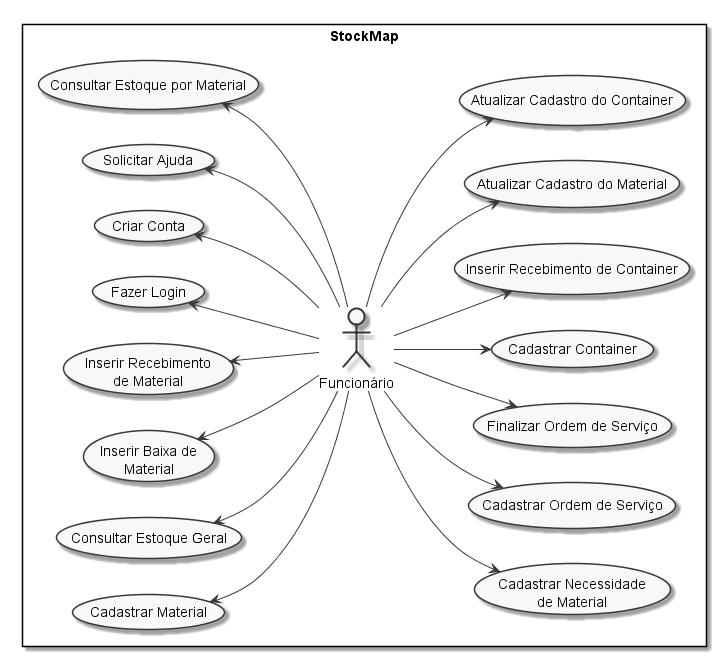
\includegraphics[width=\textwidth]{./Images/Casos_de_Uso.png}
    \caption{Diagrama de Casos de Uso}
    \label{fig:diag_caso_uso}
\end{figure}

\subsection{Descritivos de Caso de Uso}

A definição dos casos de uso somente será considerada completa uma vez que são definidos os fluxos de execução de cada caso de uso criado no primeiro diagrama.

A seguir estão expostas as 15 descrições de fluxo de execução para cada funcionalidade do sistema, contemplando os fluxos principais e alternativos para cada uma das atividades.

\subsubsection{Cadastrar Material}

\begin{figure}[H]
    \centering
    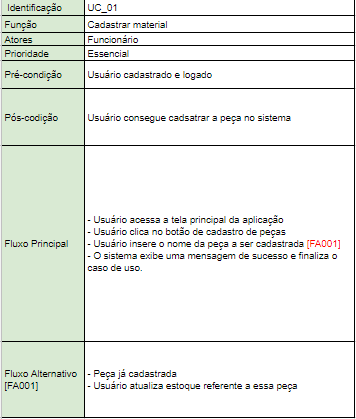
\includegraphics[scale=0.6, width=300pt]{./Images/Descritivos/UC1.png}
    \caption{Descritivo de Caso de Uso 1}
    \label{fig:desc_uc1}
\end{figure}

\subsubsection{Consultar Estoque Geral}

\begin{figure}[H]
    \centering
    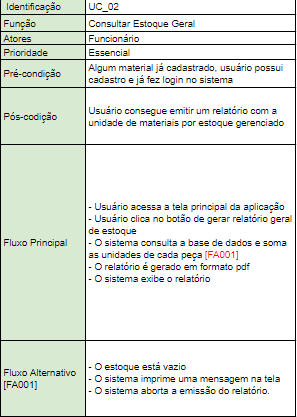
\includegraphics[scale=0.6, width=300pt]{./Images/Descritivos/UC2.png}
    \caption{Descritivo de Caso de Uso 2}
     \label{fig:desc_uc2}
\end{figure}

\subsubsection{Inserir Baixa de Material}

\begin{figure}[H]
    \centering
    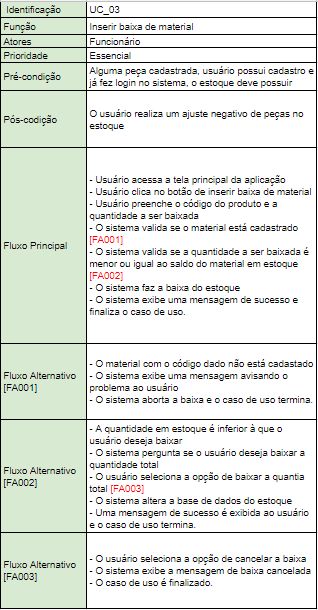
\includegraphics[scale=0.6, width=300pt]{./Images/Descritivos/UC3.png}
    \caption{Descritivo de Caso de Uso 3}
     \label{fig:desc_uc3}
\end{figure}

\subsubsection{Inserir Recebimento de Material}

\begin{figure}[H]
    \centering
    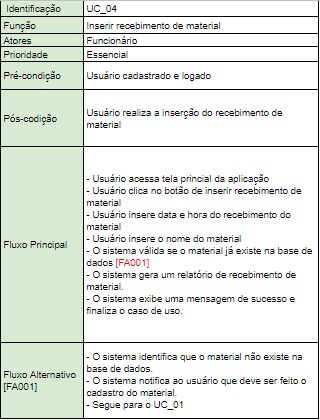
\includegraphics[scale=0.6, width=300pt]{./Images/Descritivos/UC4.png}
    \caption{Descritivo de Caso de Uso 4}
     \label{fig:desc_uc4}
\end{figure}

\subsubsection{Fazer Login}

\begin{figure}[H]
    \centering
    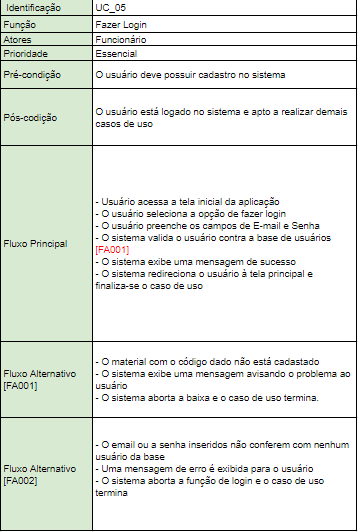
\includegraphics[scale=0.6, width=300pt]{./Images/Descritivos/UC5.png}
    \caption{Descritivo de Caso de Uso 5}
     \label{fig:desc_uc5}
\end{figure}

\subsubsection{Criar Conta}

\begin{figure}[H]
    \centering
    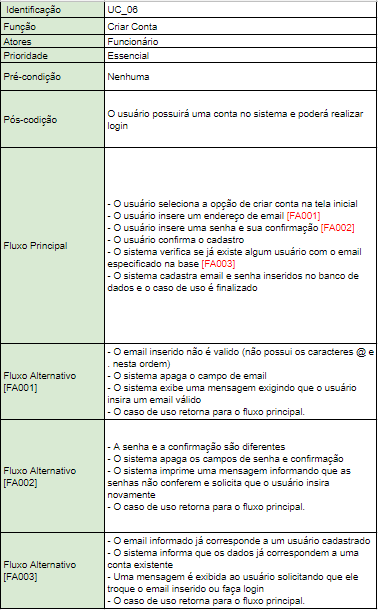
\includegraphics[scale=0.6, width=300pt]{./Images/Descritivos/UC6.png}
    \caption{Descritivo de Caso de Uso 6}
     \label{fig:desc_uc6}
\end{figure}

\subsubsection{Solicitar Ajuda}

\begin{figure}[H]
    \centering
    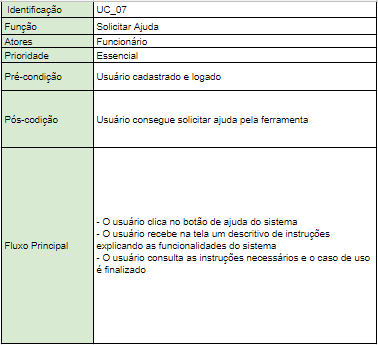
\includegraphics[scale=0.6, width=300pt]{./Images/Descritivos/UC7.png}
    \caption{Descritivo de Caso de Uso 7}
     \label{fig:desc_uc7}
\end{figure}

\subsubsection{Consultar Estoque por Material}

\begin{figure}[H]
    \centering
    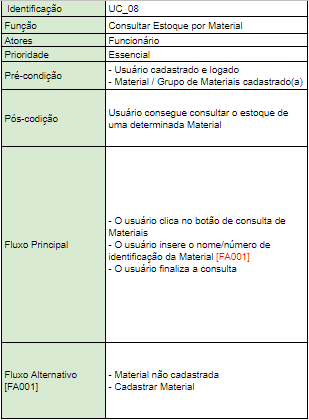
\includegraphics[scale=0.6, width=300pt]{./Images/Descritivos/UC8.png}
    \caption{Descritivo de Caso de Uso 8}
     \label{fig:desc_uc8}
\end{figure}


\subsubsection{Cadastrar Necessidade de Material}

\begin{figure}[H]
    \centering
    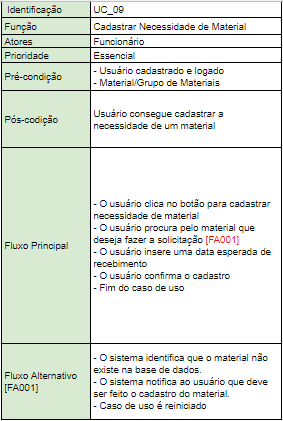
\includegraphics[scale=0.6, width=300pt]{./Images/Descritivos/UC9.png}
    \caption{Descritivo de Caso de Uso 9}
     \label{fig:desc_uc8}
\end{figure}

\subsubsection{Cadastrar Ordem de Serviço}

\begin{figure}[H]
    \centering
    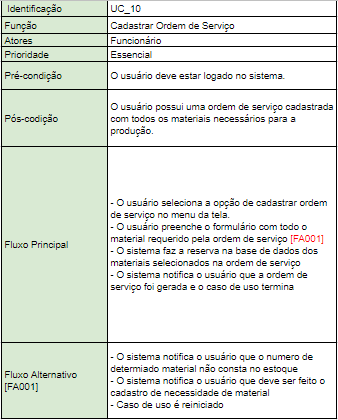
\includegraphics[scale=0.6, width=300pt]{./Images/Descritivos/UC10.png}
    \caption{Descritivo de Caso de Uso 10}
     \label{fig:desc_uc10}
\end{figure}

\subsubsection{Finalizar Ordem de Serviço}

\begin{figure}[H]
    \centering
    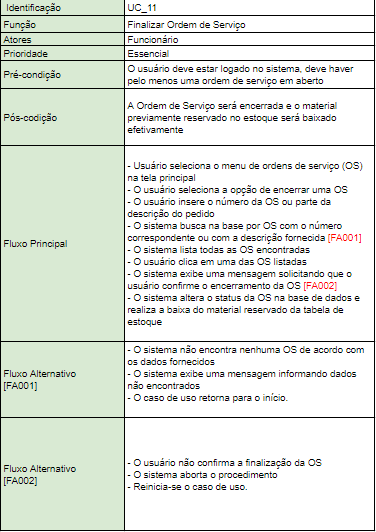
\includegraphics[scale=0.6, width=300pt]{./Images/Descritivos/UC11.png}
    \caption{Descritivo de Caso de Uso 11}
     \label{fig:desc_uc11}
\end{figure}

\subsubsection{Cadastrar Container}

\begin{figure}[H]
    \centering
    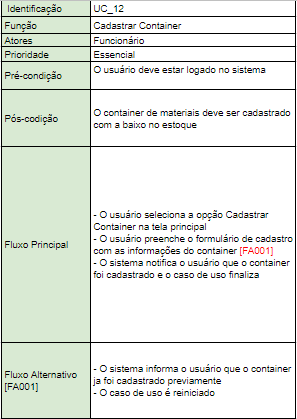
\includegraphics[scale=0.6, width=300pt]{./Images/Descritivos/UC12.png}
    \caption{Descritivo de Caso de Uso 12}
     \label{fig:desc_uc12}
\end{figure}

\subsubsection{Inserir Recebimento de Container}

\begin{figure}[H]
    \centering
    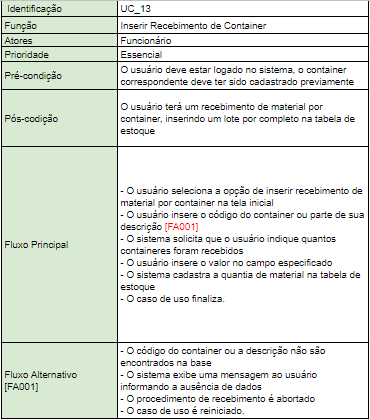
\includegraphics[scale=0.6, width=300pt]{./Images/Descritivos/UC13.png}
    \caption{Descritivo de Caso de Uso 13}
     \label{fig:desc_uc13}
\end{figure}

\subsubsection{Atualizar Cadastro do Material}

\begin{figure}[H]
    \centering
    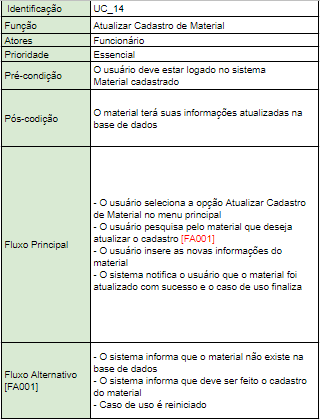
\includegraphics[scale=0.6, width=300pt]{./Images/Descritivos/UC14.png}
    \caption{Descritivo de Caso de Uso 14}
     \label{fig:desc_uc14}
\end{figure}

\subsubsection{Atualizar Cadastro do Container}

\begin{figure}[H]
    \centering
    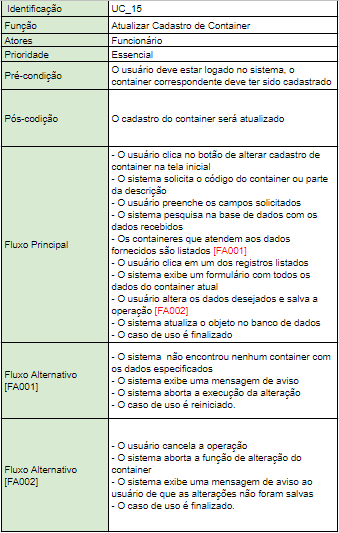
\includegraphics[scale=0.6, width=300pt]{./Images/Descritivos/UC15.png}
    \caption{Descritivo de Caso de Uso 15}
     \label{fig:desc_uc15}
\end{figure}

\section{Diagrama de Classes} \label{diagramaClasse}

O diagrama de classes é um dos diagramas mais importantes dentro da UML. Esse serve de apoio para a grande maioria dos demais diagramas. Esse diagrama trás a representação das classes do sistema, acompanhado de seus atributos e métodos, e seus relacionamentos e troca de informações. Abaixo encontra-se a representação do Diagrama de Classes desenvolvido:

\begin{landscape}
    \begin{figure}
    \centering
      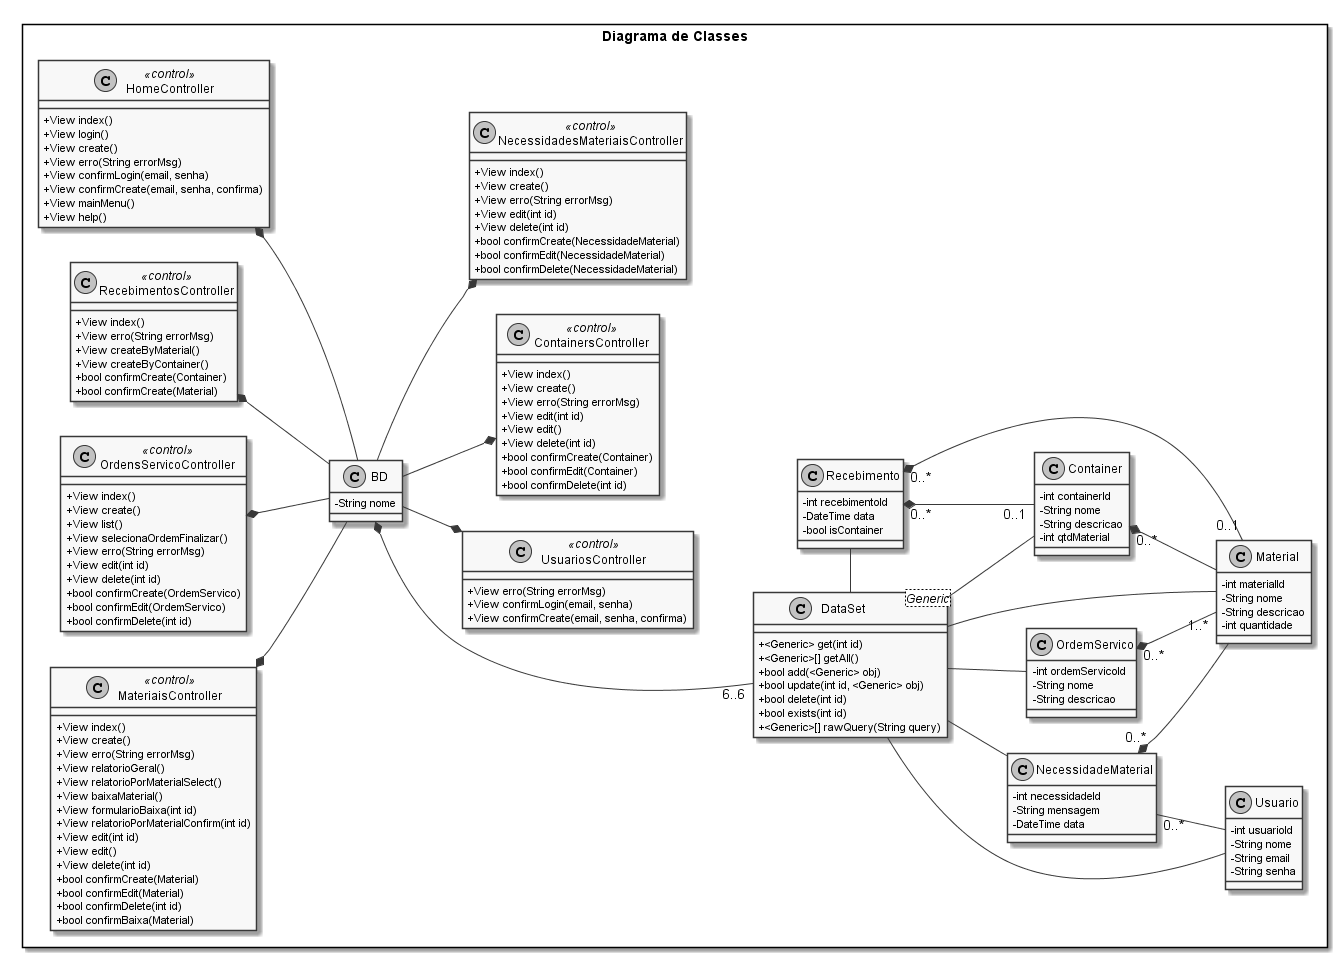
\includegraphics[scale=0.6, width=650pt]{./Images/Classes.png}
      \caption{Diagrama de Classes}
      \label{fig:DS_Gerente16}
      \end{figure}
\end{landscape}

Esse diagrama foi modelado visando o uso do padrão MVC (Model, View, Controller), onde a Model representa as entidades do sistema, a View as páginas de interface com o usuário e por final a Controller, onde a lógica de négocio do sistema é representada e executada. Algumas classes do diagrama tem um propósito generalista, como a "DataSet", que consegue trabalhar todas as entidades do modelo, outra é a classe "BD" que tem relacionamento com todas as Controllers, como também com a classe "Dataset".

\newpage

\section{Diagrama de Sequência} \label{diagramaSeq}

O Diagrama de Sequência é costumeiramente projetado após a definição dos diagramas de casos de uso e de sequência, este é modelado para representar de forma cronológica a troca de mensagens entre cada componente do sistema, podendo estes componentes serem os atores, as interfaces ou os controladores projetados.

Abaixo são exibidos os 15 diagramas que exemplificam a troca de mensagens executadas para o funcionamento normal do sistema bem como os fluxos alternativos de execução definidos na etapa de descrição dos casos de uso da plataforma.

\subsection{Cadastrar Material}

\begin{figure}[H]
    \centering
    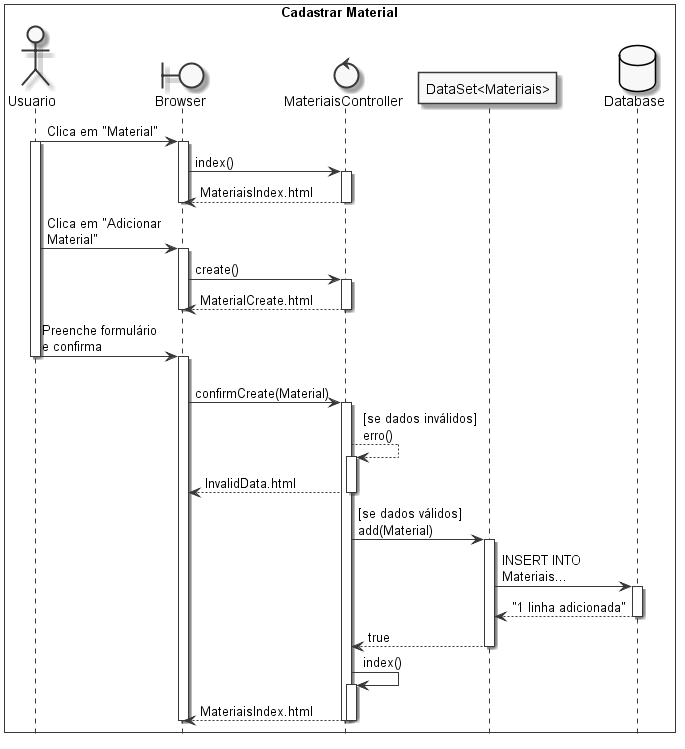
\includegraphics[scale=0.6, width=395pt]{./Images/DS_Cadastrar_Material.jpg}
    \caption{Diagrama de Sequencia 1}
    \label{fig:diag_seq1}
\end{figure}

\subsection{Consultar Estoque Geral}

\begin{figure}[H]
    \centering
    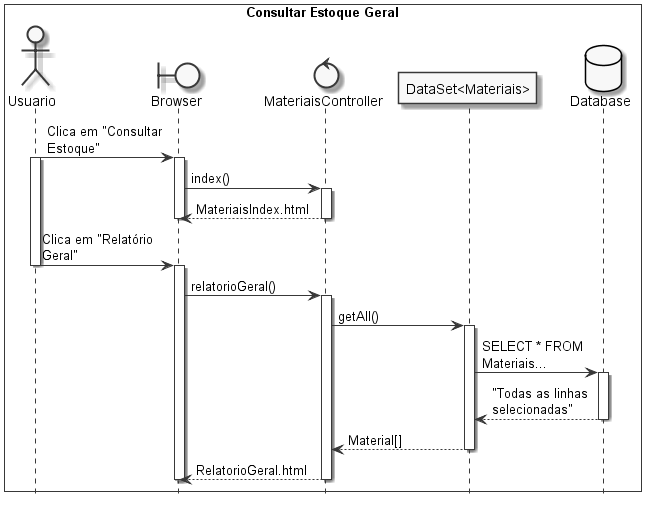
\includegraphics[width=\textwidth]{./Images/DS_Consultar_Estoque_Geral.jpg}
    \caption{Diagrama de Sequencia 2}
    \label{fig:diag_seq2}
\end{figure}

\subsection{Inserir Baixa de Material}

\begin{figure}[H]
    \centering
    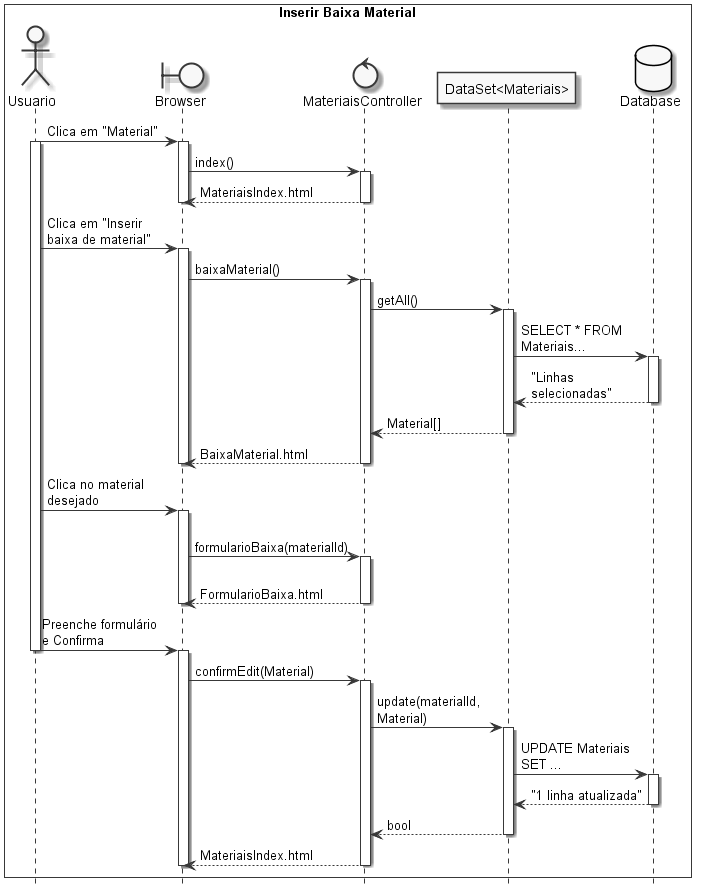
\includegraphics[width=\textwidth]{./Images/DS_Inserir_Baixa_Material.jpg}
    \caption{Diagrama de Sequencia 3}
    \label{fig:diag_seq3}
\end{figure}

\subsection{Inserir Recebimento de Material}

\begin{figure}[H]
    \centering
    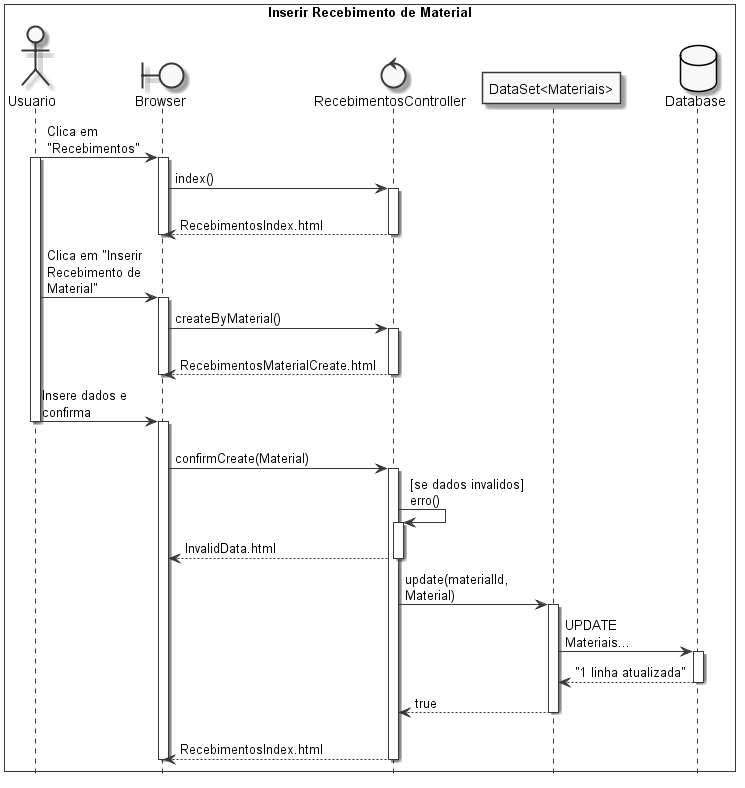
\includegraphics[width=\textwidth]{./Images/DS_Inserir_Recebimento_Material.jpg}
    \caption{Diagrama de Sequencia 4}
    \label{fig:diag_seq4}
\end{figure}

\subsection{Fazer Login}

\begin{figure}[H]
    \centering
    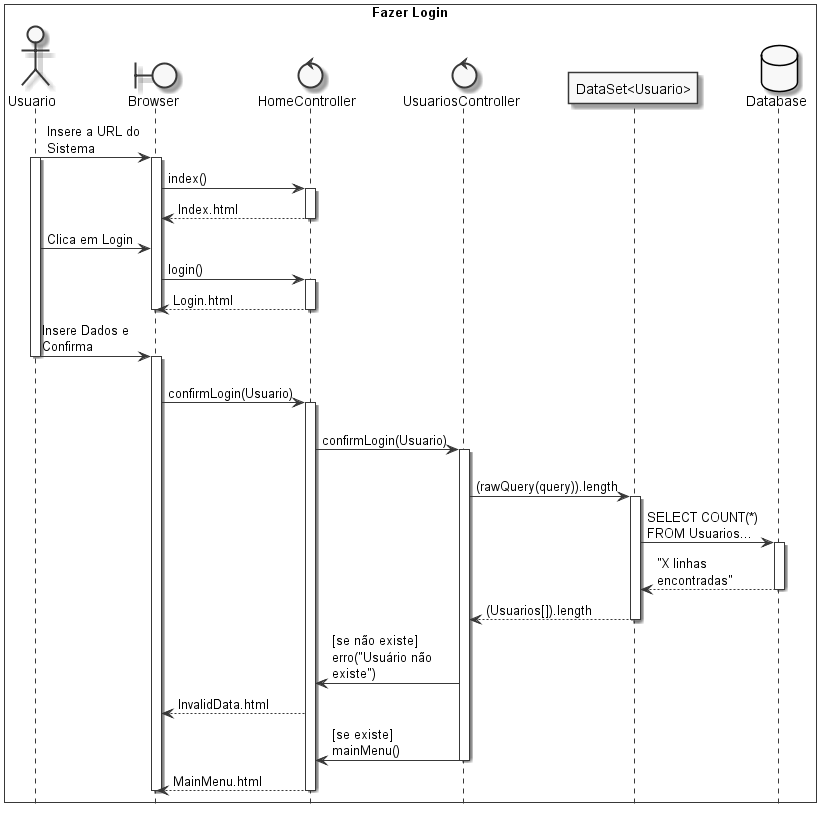
\includegraphics[width=\textwidth]{./Images/DS_Fazer_Login.jpg}
    \caption{Diagrama de Sequencia 5}
    \label{fig:diag_seq5}
\end{figure}

\subsection{Criar Conta}

\begin{figure}[H]
    \centering
    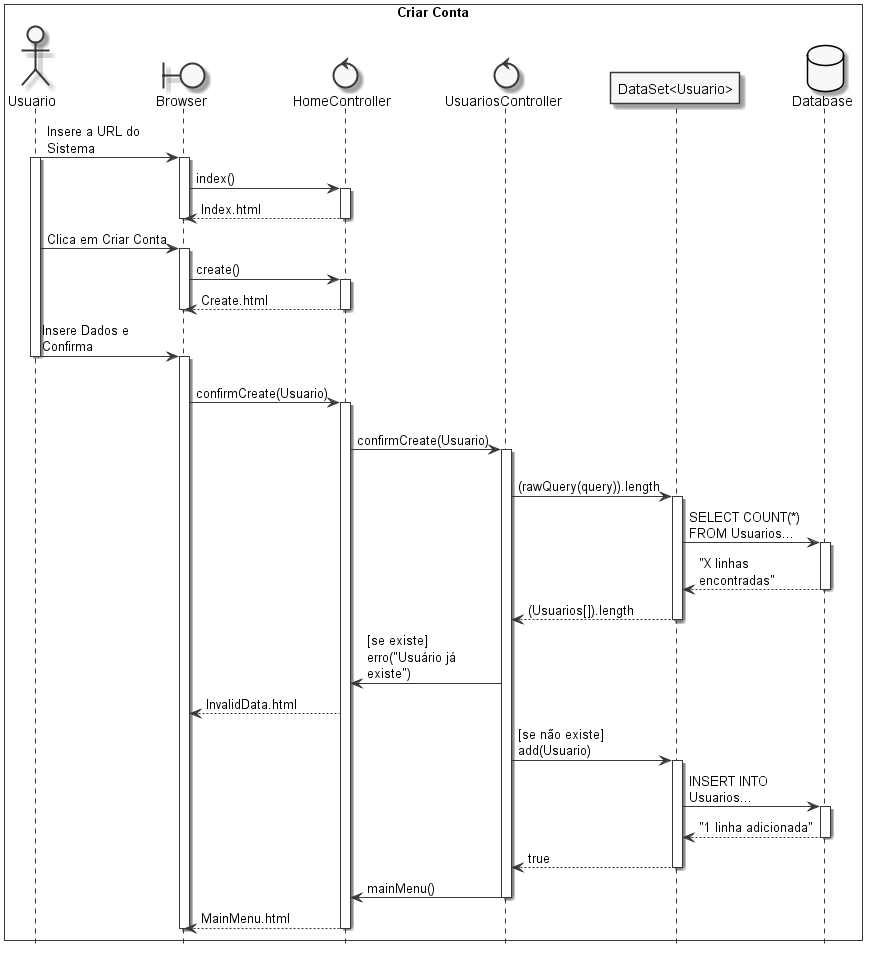
\includegraphics[width=\textwidth]{./Images/DS_Criar_Conta.jpg}
    \caption{Diagrama de Sequencia 6}
    \label{fig:diag_seq6}
\end{figure}

\subsection{Solicitar Ajuda}

\begin{figure}[H]
    \centering
    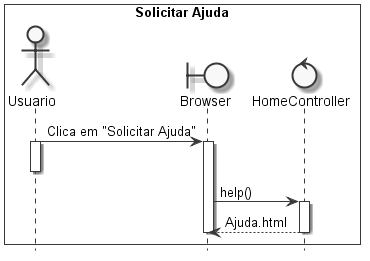
\includegraphics[width=\textwidth]{./Images/DS_Solicitar_Ajuda.jpg}
    \caption{Diagrama de Sequencia 7}
    \label{fig:diag_seq7}
\end{figure}

\subsection{Consultar Estoque por Material}

\begin{figure}[H]
    \centering
    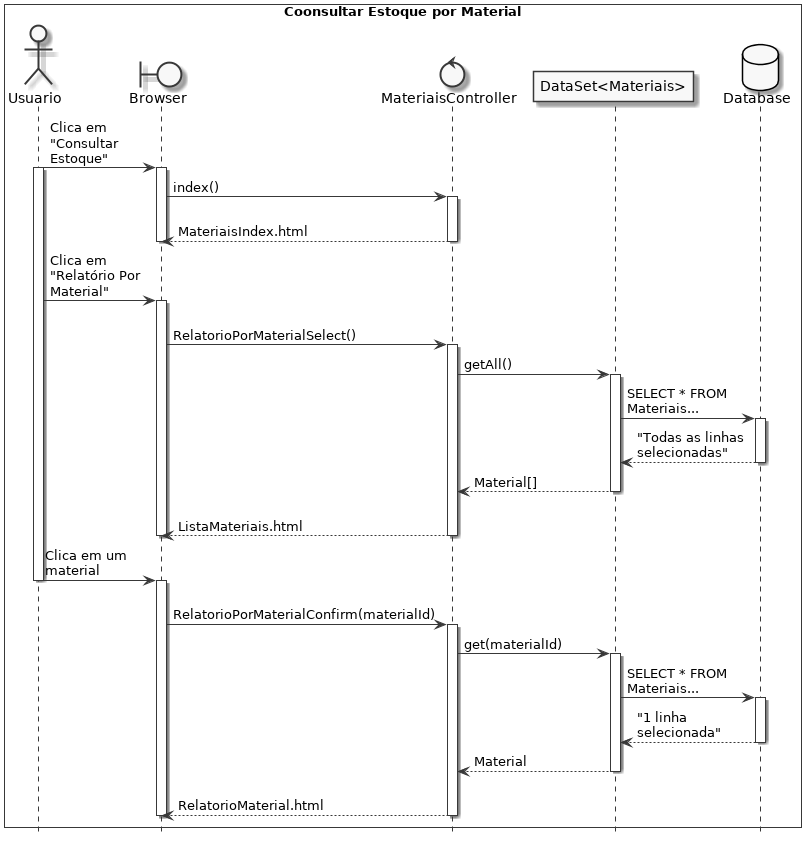
\includegraphics[width=\textwidth]{./Images/DS_Consultar_Estoque_Material.png}
    \caption{Diagrama de Sequencia 8}
    \label{fig:diag_seq8}
\end{figure}

\subsection{Cadastrar Necessidade de Material}

\begin{figure}[H]
    \centering
    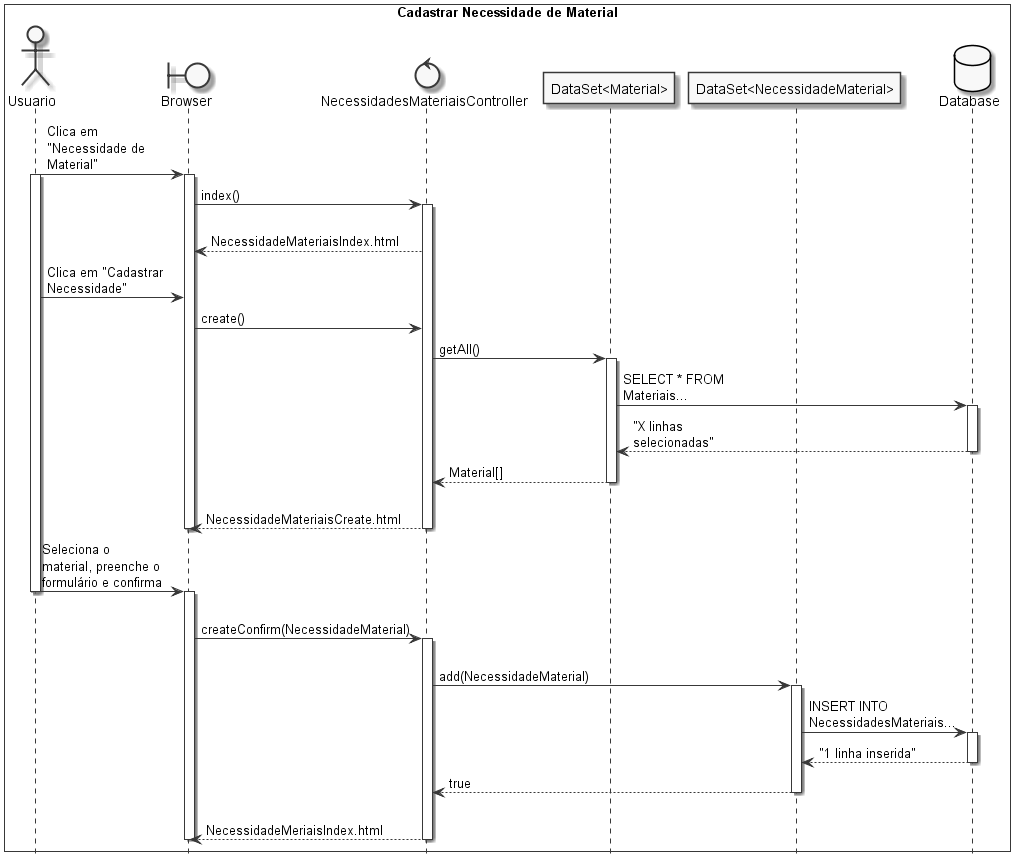
\includegraphics[width=\textwidth]{./Images/DS_Cadastrar_Necessidade_Material.jpg}
    \caption{Diagrama de Sequencia 9}
    \label{fig:diag_seq9}
\end{figure}

\subsection{Cadastrar Ordem de Serviço}

\begin{figure}[H]
    \centering
    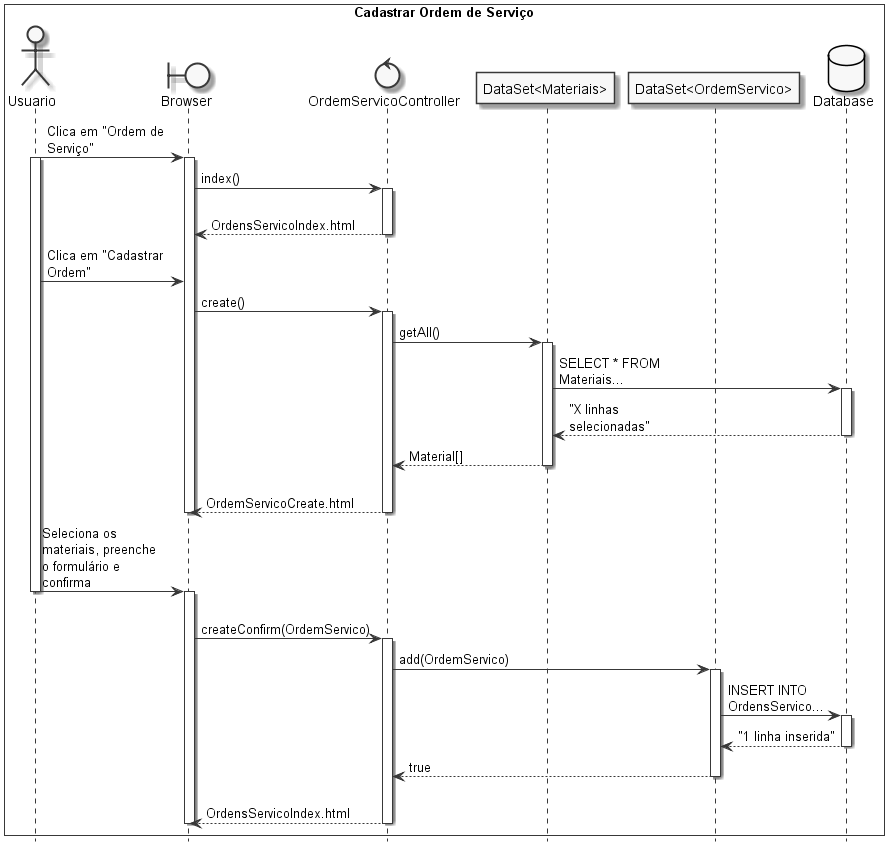
\includegraphics[scale=0.6, width=400pt]{./Images/DS_Cadastrar_Ordem_Servico.jpg}
    \caption{Diagrama de Sequencia 10}
    \label{fig:diag_seq10}
\end{figure}

\subsection{Finalizar Ordem de Serviço}

\begin{figure}[H]
    \centering
    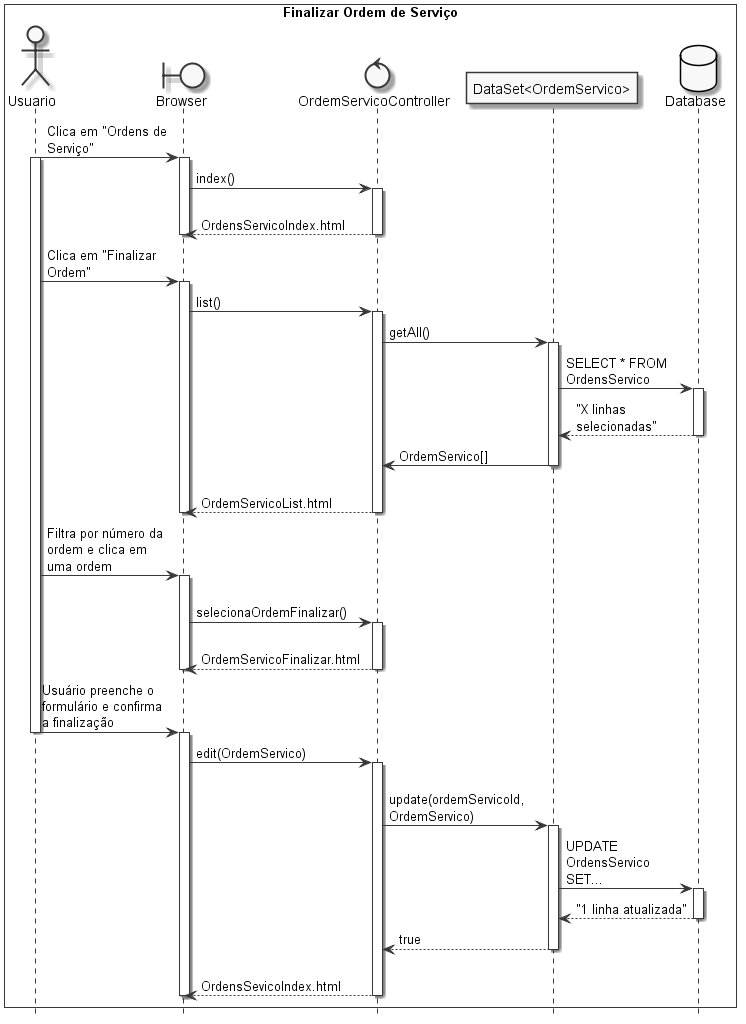
\includegraphics[width=\textwidth]{./Images/DS_Finalizar_Ordem_Servico.jpg}
    \caption{Diagrama de Sequencia 11}
    \label{fig:diag_seq11}
\end{figure}

\subsection{Cadastrar Container}

\begin{figure}[H]
    \centering
    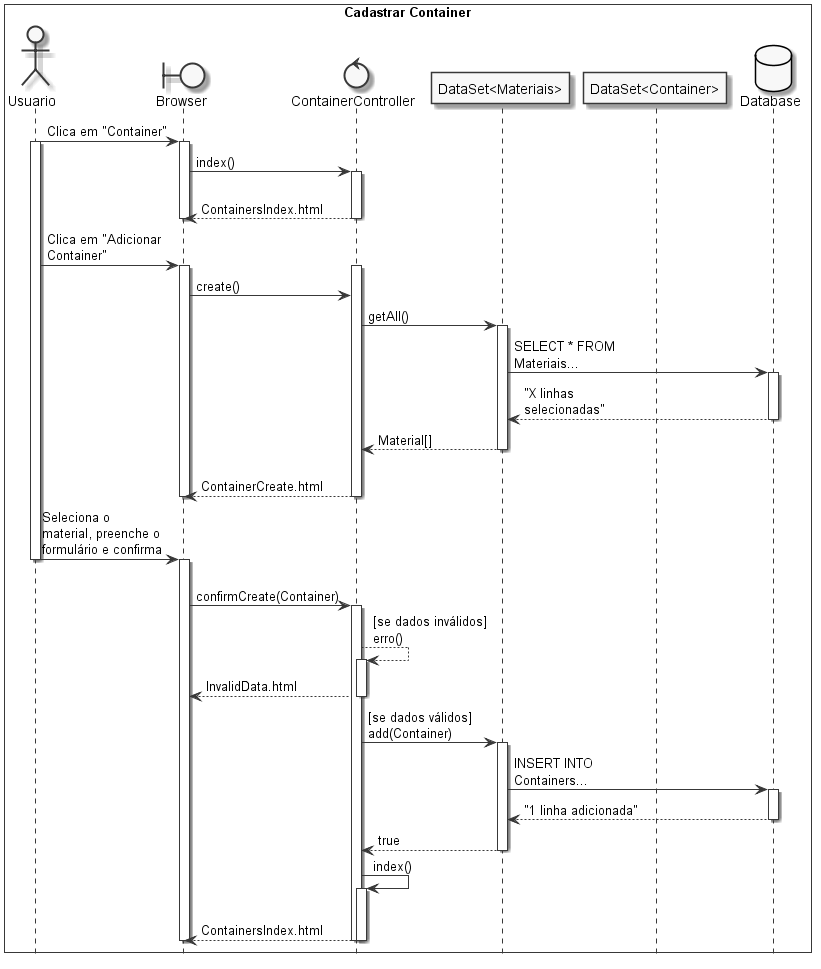
\includegraphics[width=\textwidth]{./Images/DS_Cadastrar_Container.jpg}
    \caption{Diagrama de Sequencia 12}
    \label{fig:diag_seq12}
\end{figure}

\subsection{Inserir Recebimento de Container}

\begin{figure}[H]
    \centering
    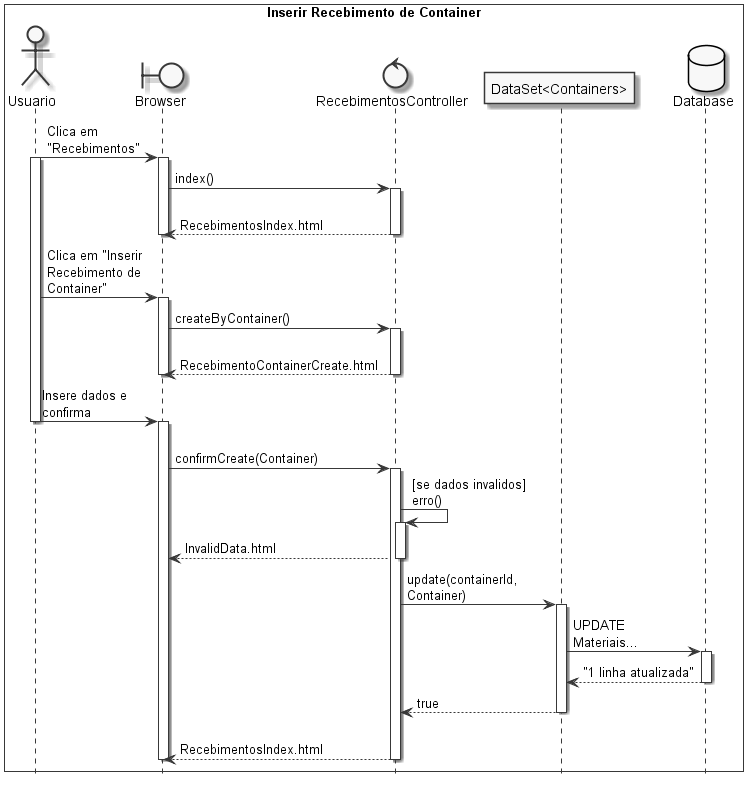
\includegraphics[width=\textwidth]{./Images/DS_Inserir_Recebimento_Container.jpg}
    \caption{Diagrama de Sequencia 13}
    \label{fig:diag_seq13}
\end{figure}

\subsection{Atualizar Cadastro do Material}

\begin{figure}[H]
    \centering
    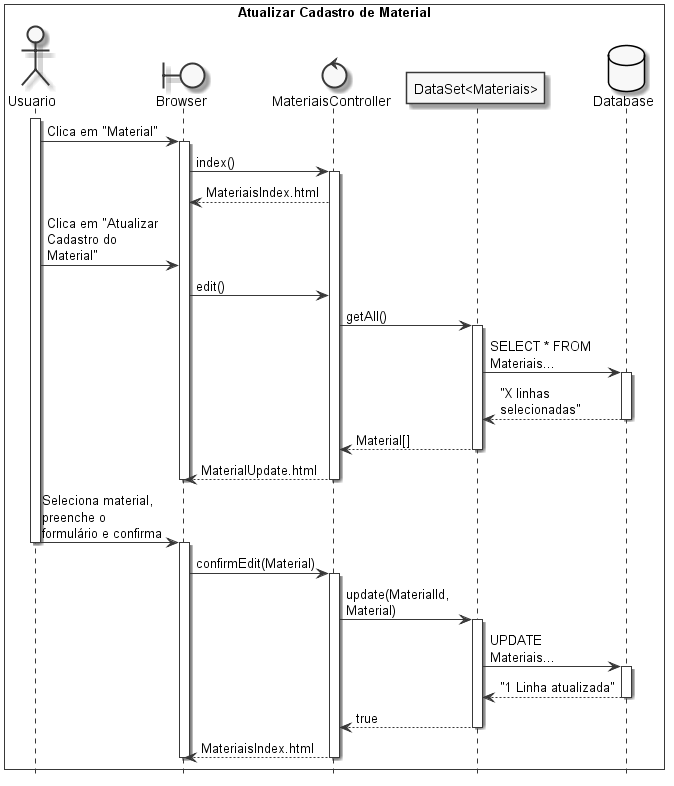
\includegraphics[width=\textwidth]{./Images/DS_Atualizar_Cadastro_Material.jpg}
    \caption{Diagrama de Sequencia 14}
    \label{fig:diag_seq14}
\end{figure}

\subsection{Atualizar Cadastro do Container}

\begin{figure}[H]
    \centering
    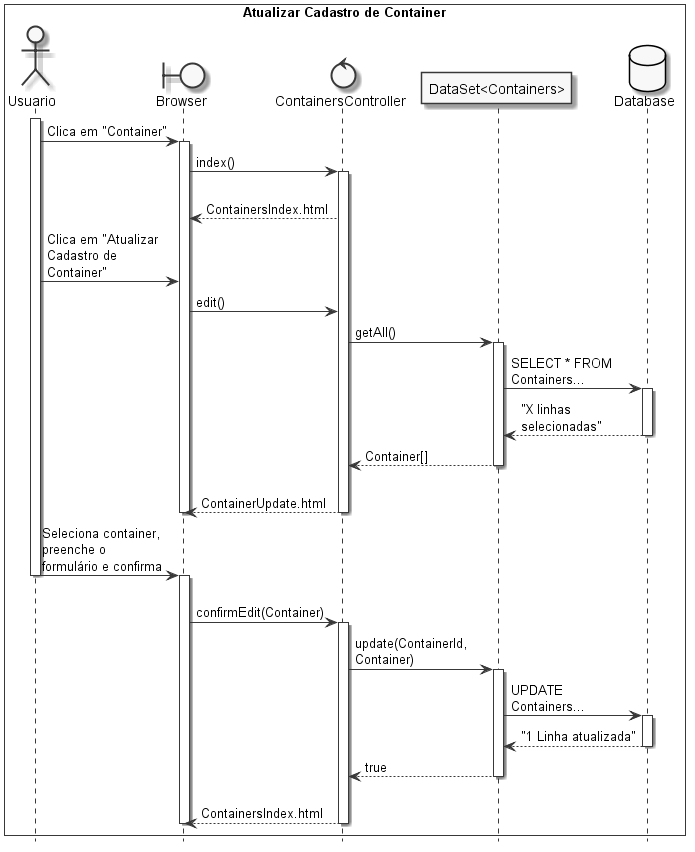
\includegraphics[width=\textwidth]{./Images/DS_Atualizar_Cadastro_Container.jpg}
    \caption{Diagrama de Sequencia 15}
    \label{fig:diag_seq15}
\end{figure}

\newpage

\section{Diagrama de Estados} \label{diagramaEstados}

O Diagrama de Estados representa o comportamento de um elemento por meio de diversas transições de estado, ou seja, uma máquina de estados. Esse diagrama muitas vezes é utilizado para expressar o comportamento de uma parte do sistema, que pode ser representado por um caso de uso. Nesse trabalho os Diagramas de Estados foram segmentados por Casos de Uso [\ref{diagramaCasoUso}], onde cada caso de uso tem uma determinada sequência de estados, até atingir seu término. As sub-seções abaixo ilustram e descrevem cada Diagrama de Estado.

\subsection{Cadastrar Material}

Nesse diagrama é representado o os estados da classe MateriaisController, que nesse diagrama se responsabiliza por cadastrar um Material no final de sua execuação. O diagrama decorre sobre a atuação do Usuário que utiliza um Browser para fazer requisições e processar as Views retornadas pela Controller. O usuário deve preencher um formulário e confirmar os dados que serão enviados para o banco de dados para a criação de um novo material, mas antes de sua persistência o sistema valida a existência de um material igual ao que está senda cadastrado, evitando redundância.


\begin{figure}[H]
    \centering
    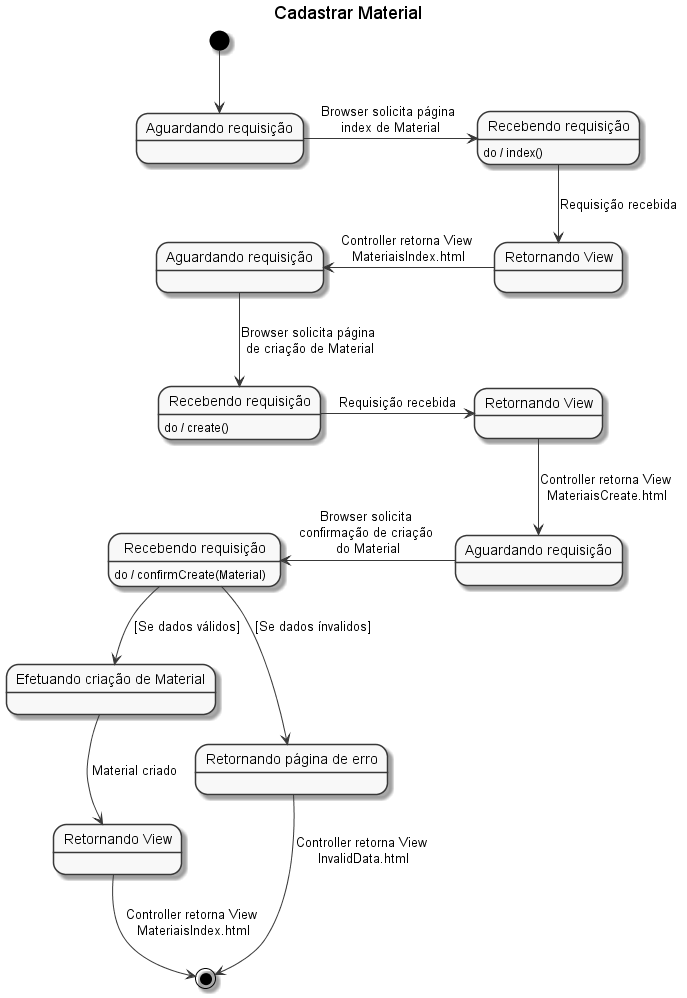
\includegraphics[scale=0.6, width=400pt]{./Images/DE_-_Cadastrar_Material.png}
    \caption{Diagrama de Estados 1}
    \label{fig:diag_est1}
\end{figure}

\pagebreak

\subsection{Consultar Estoque Geral}

Neste Diagrama de Estados é representado o comportamento da classe MateriaisController, a qual é responsável por receber a requisição do usuário, através do Browser, para emissão do relatório de estoque geral, então uma solicitação é enviada ao Banco de Dados para geração do dataset com os dados de todo o estoque. Após o recebimento dos dados por parte do controller a página do relatório é renderizada no servidor e enviada novamente ao Browser.

\begin{figure}[H]
    \centering
    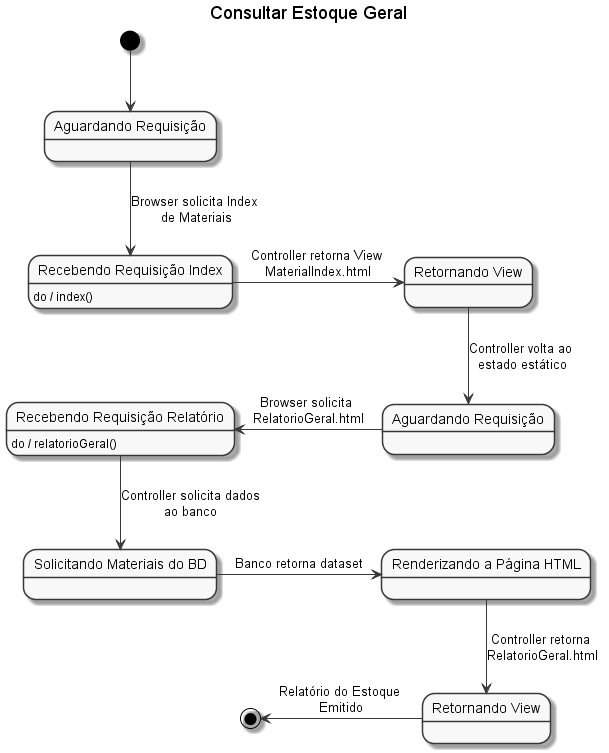
\includegraphics[scale=0.6, width=400pt]{./Images/DE_-_Consultar_Estoque_Geral.png}
    \caption{Diagrama de Estados 2}
    \label{fig:diag_est2}
\end{figure}

\subsection{Inserir Baixa de Material}

Neste diagrama a classe responsável por tratar as requisições é a MateriaisController, a qual deve devolver ao Browser os formulários de baixa de materiais e, ao recebê-lo preenchido, validar os dados retornados, enviando para o Banco de Dados uma atualização negativa caso as informações sejam válidas, assim ajustando o estoque.

\begin{figure}[H]
    \centering
    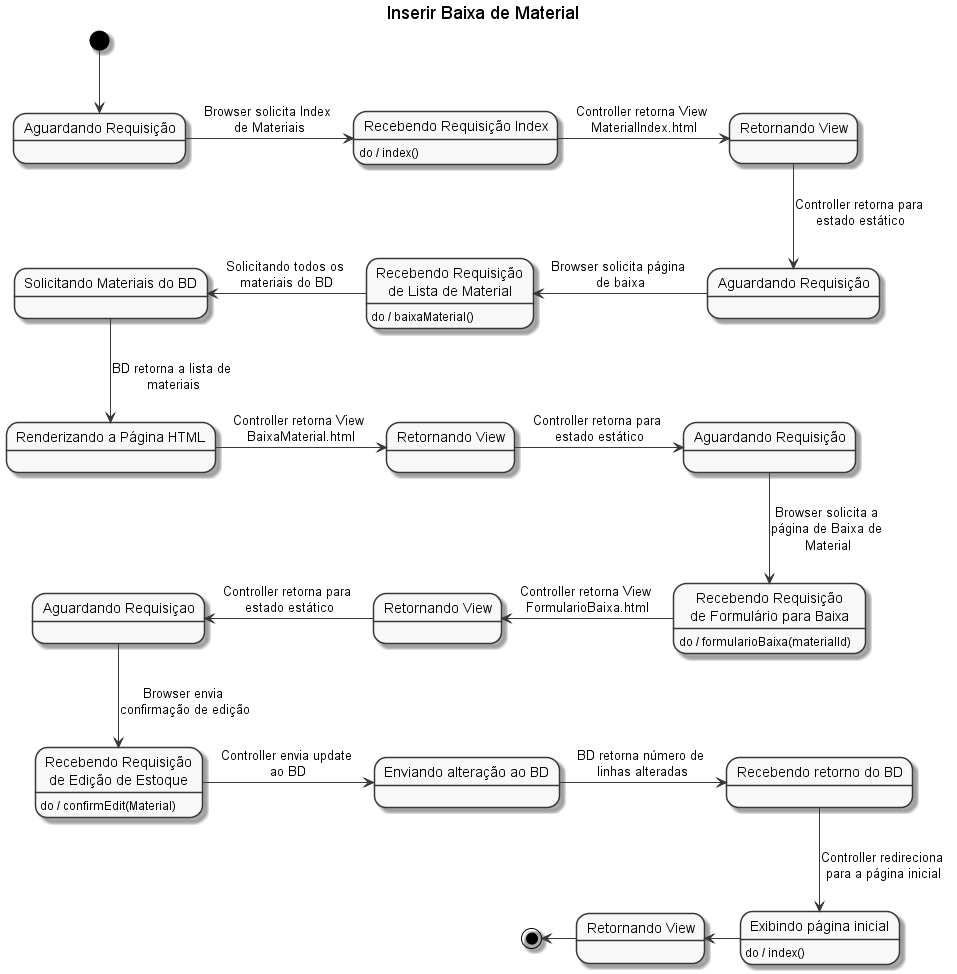
\includegraphics[width=\textwidth]{./Images/DE_-_Inserir_Baixa_de_Material.png}
    \caption{Diagrama de Estados 3}
    \label{fig:diag_est3}
\end{figure}

\subsection{Inserir Recebimento de Material}

Neste diagrama a classe responsável por tratar as requisições é a MateriaisController, a qual deve retornar para o usuário o formulário de recebimento de materiais, validar os dados enviados pelo Browser e então, somente se as informações estiverem corretas, enviar ao Banco de Dados uma solicitação de incremento de saldo para o material informado pelo usuário.

\begin{figure}[H]
    \centering
    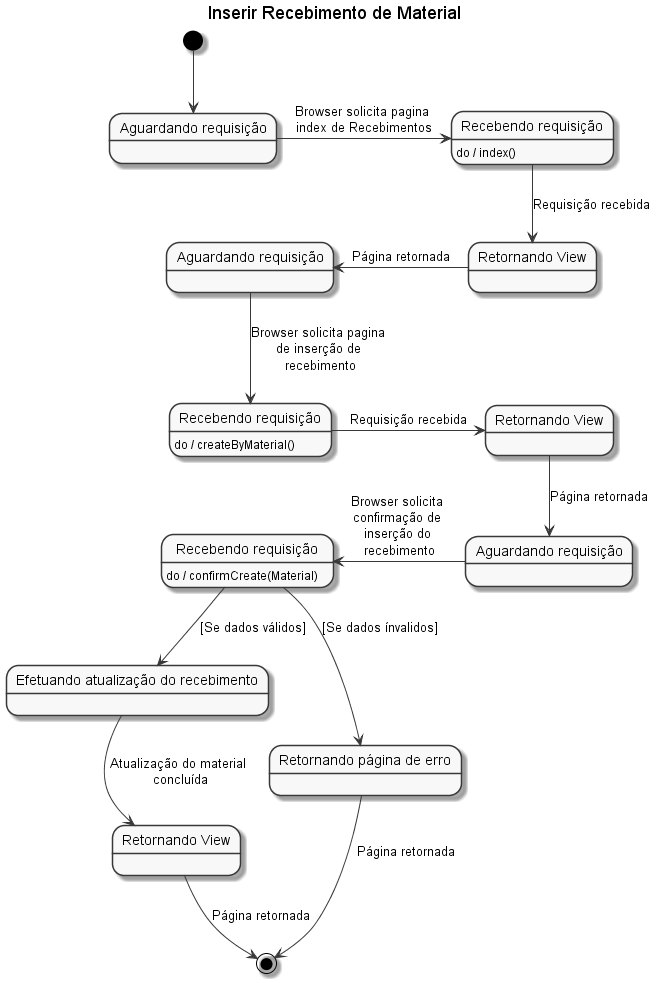
\includegraphics[scale=0.6, width=400pt]{./Images/DE_-_Inserir_Recebimento_de_Material.png}
    \caption{Diagrama de Estados 4}
    \label{fig:diag_est4}
\end{figure}

\subsection{Fazer Login}

A classe responsável por este diagrama é a HomeController. Neste caso, o usuário seleciona na tela inicial a opção de realizar login, o controlador deve retornar o formulário de acesso e validar os dados preenchidos após seu recebimento. Caso os dados estejam de acordo com o existente no banco de dados o controlador redireciona o usuário ao menu inicial da aplicação.

\begin{figure}[H]
    \centering
    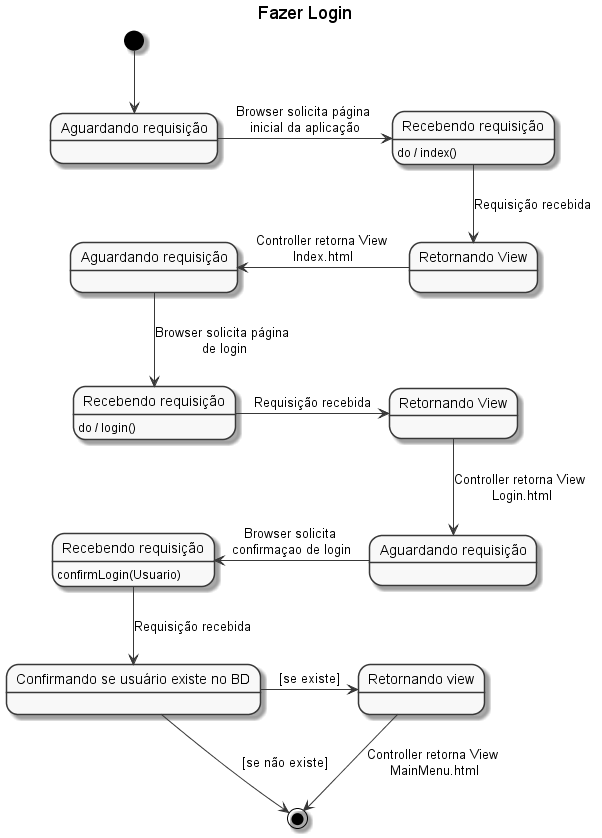
\includegraphics[scale=0.6, width=350pt]{./Images/DE_-_Fazer_Login.png}
    \caption{Diagrama de Estados 5}
    \label{fig:diag_est5}
\end{figure}

\subsection{Criar Conta}

Neste diagrama de estados o controlador HomeController deve receber a solicitação do usuário, fornecer o formulário de cadastro do sistema, então, após seu preenchimento deve-se validar frente ao banco se as informações são válidas e, caso sejam, o controlador envia a solicitação de cadastro do usuário na base de dados e o redireciona para a página inicial do sistema.

\begin{figure}[H]
    \centering
    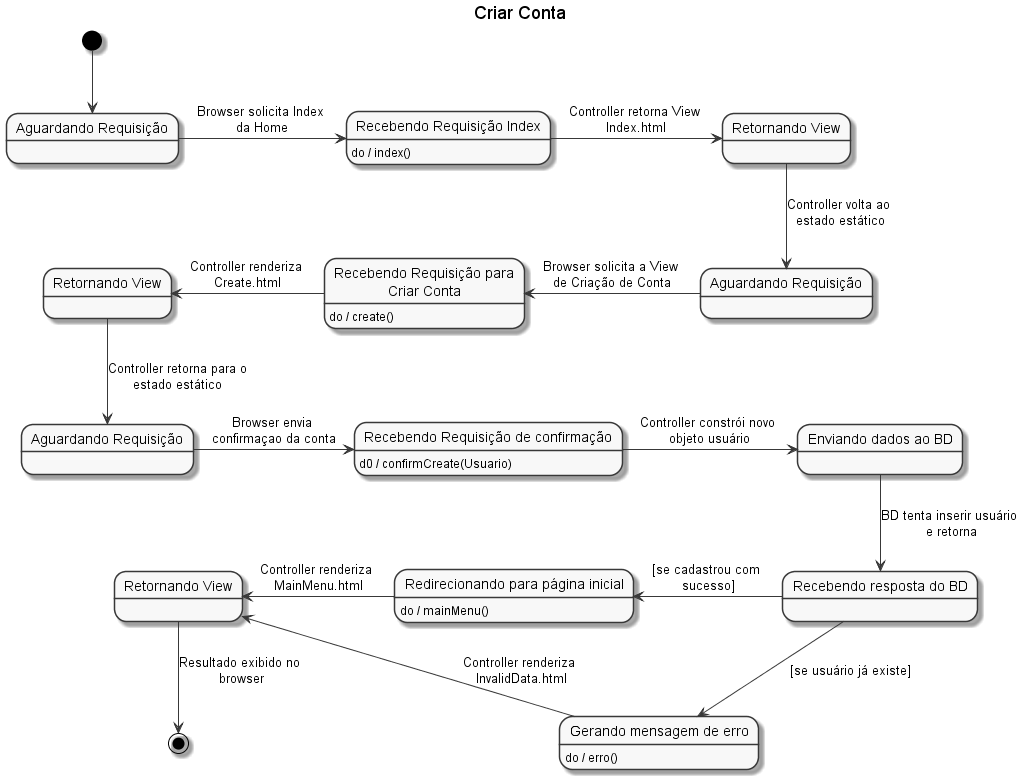
\includegraphics[width=\textwidth]{./Images/DE_-_Criar_Conta.png}
    \caption{Diagrama de Estados 6}
    \label{fig:diag_est6}
\end{figure}

\subsection{Solicitar Ajuda}

Esse diagrama modela o comportamento do HomeController, que recebe uma requisição do Browser para processar o menu de ajuda para o usuário.

\begin{figure}[H]
    \centering
    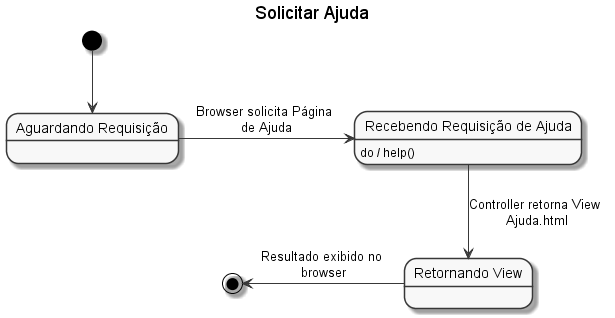
\includegraphics[width=\textwidth]{./Images/DE_-_Solicitar_Ajuda.png}
    \caption{Diagrama de Estados 7}
    \label{fig:diag_est7}
\end{figure}


\subsection{Consultar Estoque por Material}

O controlador representado neste diagrama é o MateriaisController, neste caso o usuário deve solicitar a lista de materiais e, após seu recebimento, selecionar um material para visualização do saldo em estoque. O controlador então trata a requisição e solicita ao Banco de Dados um dataset com informações do material recebido. Após o retorno do dataset a página do relatório é renderizada no servidor e enviada ao Browser.

\begin{figure}[H]
    \centering
    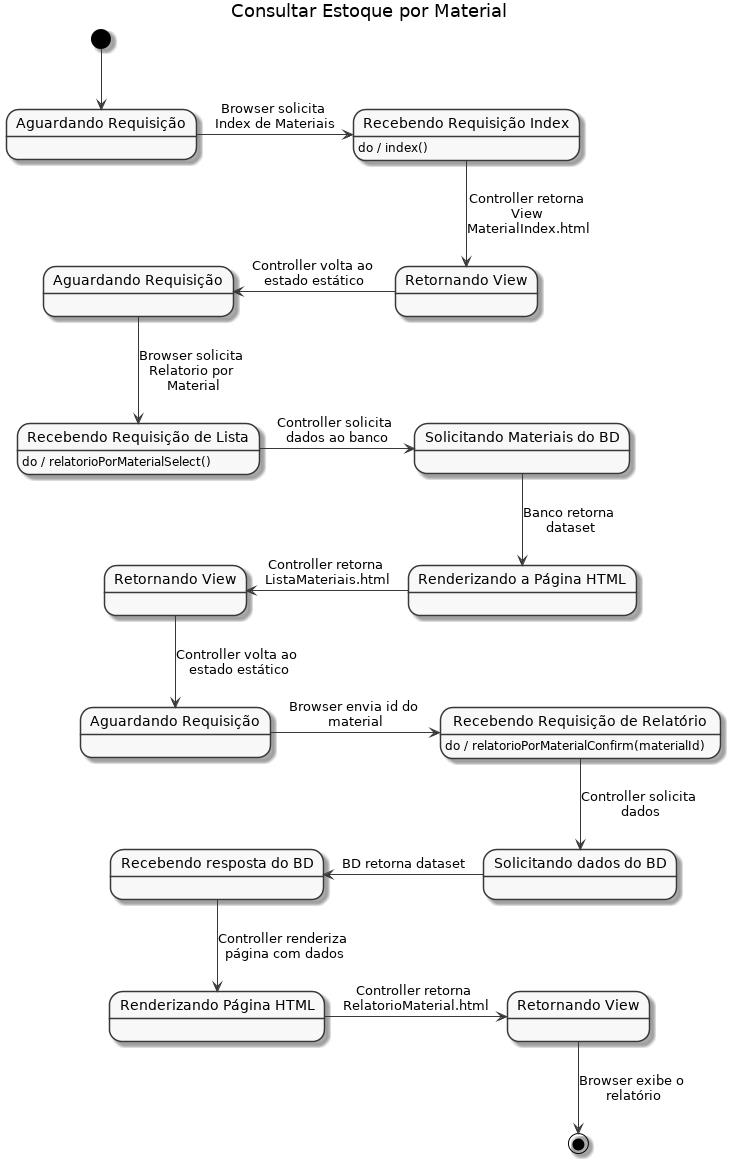
\includegraphics[scale=0.6, width=400pt]{./Images/DE_Consultar_Estoque_Material.png}
    \caption{Diagrama de Estados 8}
    \label{fig:diag_est8}
\end{figure}


\subsection{Cadastrar Necessidade de Material}

Esse diagrama apresenta o comportamento da classe MateriaisController, que nesse caso o usuário irá selecionar o material que deseja cadastrar e gerar uma alerta de necessidade, depois de selecionado o sistema irá renderizar um formulário de cadastro que será retornado para usuário pelo controller. Após o preenchimento desse formulário, o usuário confirmará o cadastro, o controller irá processar a persistência desse novo cadastro no banco de dados.

\begin{figure}[H]
    \centering
    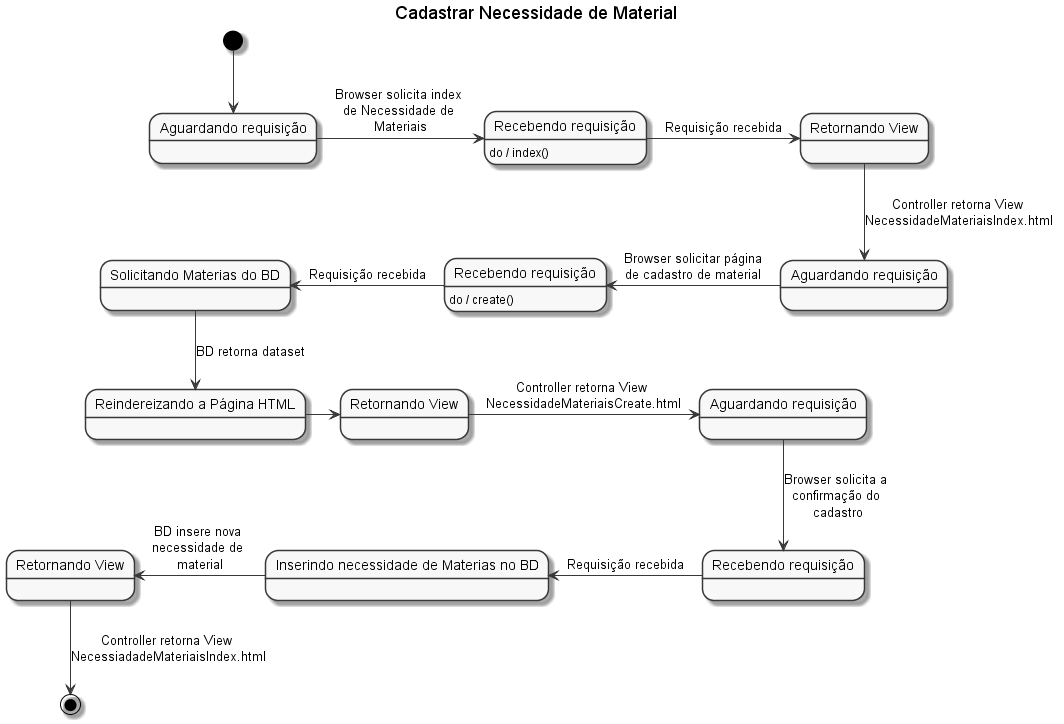
\includegraphics[width=\textwidth]{./Images/DE_-_Cadastrar_Necessidade_de_Material.png}
    \caption{Diagrama de Estados 9}
    \label{fig:diag_est9}
\end{figure}

\subsection{Cadastrar Ordem de Serviço}

Este diagrama representa o comportamento da classe OrdensServicoController, a qual deve, ao receber a solicitação do usuário, listar todos os materiais cadastrados no banco, após a seleção dos materiais desejados e suas respectivas quantidades por parte do usuário, o controlador por fim deve registrar no banco os dados informados, caso sejam inferiores aos estoques disponíveis.

\begin{figure}[H]
    \centering
    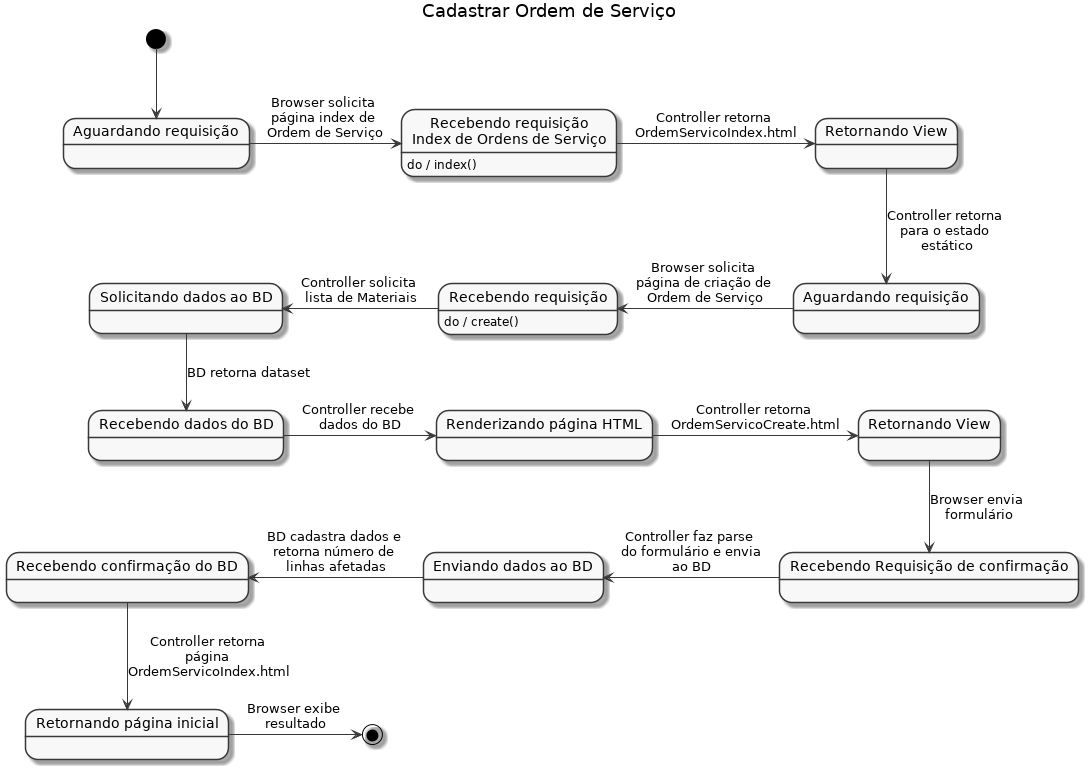
\includegraphics[width=\textwidth]{./Images/DE_Cadastrar_Ordem_Servico.png}
    \caption{Diagrama de Estados 10}
    \label{fig:diag_est10}
\end{figure}

\subsection{Finalizar Ordem de Serviço}

Aqui foi modelado o comportamento da classe OrdemServicoController, que recebe do usuário uma solicitação para listas todas as Ordens de Serviços não finalizadas no sistema. Depois de retornada todas as Ordens de Serviços, o usuário seleciona a Ordem que deseja finalizar e faz uma requisição de confirmação para o sistema. O controller processa essa requisição e a base de dados é atualizadada com a Ordem de Serviços finalizada.

\begin{figure}[H]
    \centering
    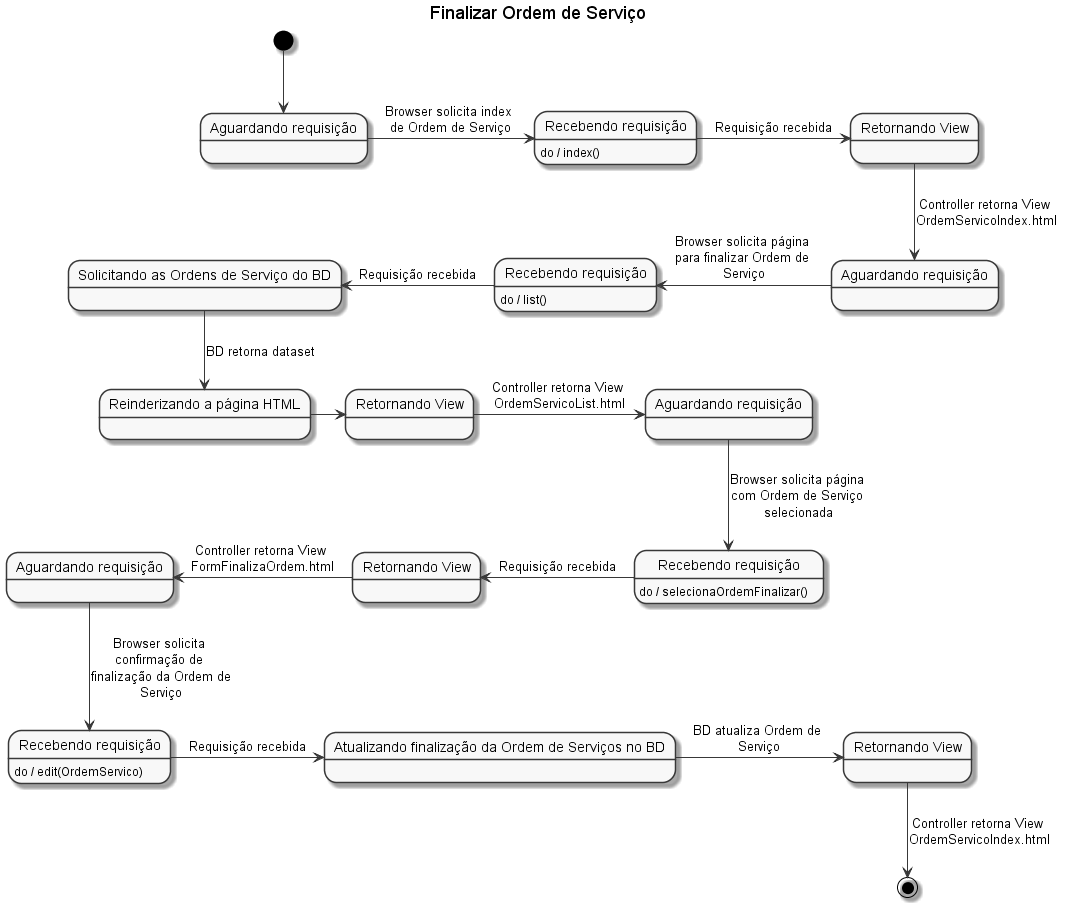
\includegraphics[width=\textwidth]{./Images/DE_-_Finalizar_Ordem_de_Servico.png}
    \caption{Diagrama de Estados 11}
    \label{fig:diag_est11}
\end{figure}


\subsection{Cadastrar Container}

Neste diagrama é representada a troca de estados do controlador ContainerController, o qual deve permitir que o usuário cadastre um agrupador de materiais para facilitar futuros cadastros de ordens de serviço e recebimentos de materiais. Após receber o material e a quantidade agrupada pelo usuário o controlador deve cadastrar no banco de dados as informações fornecidas e retornar ao usuário a página inicial do sistema novamente.

\begin{figure}[H]
    \centering
    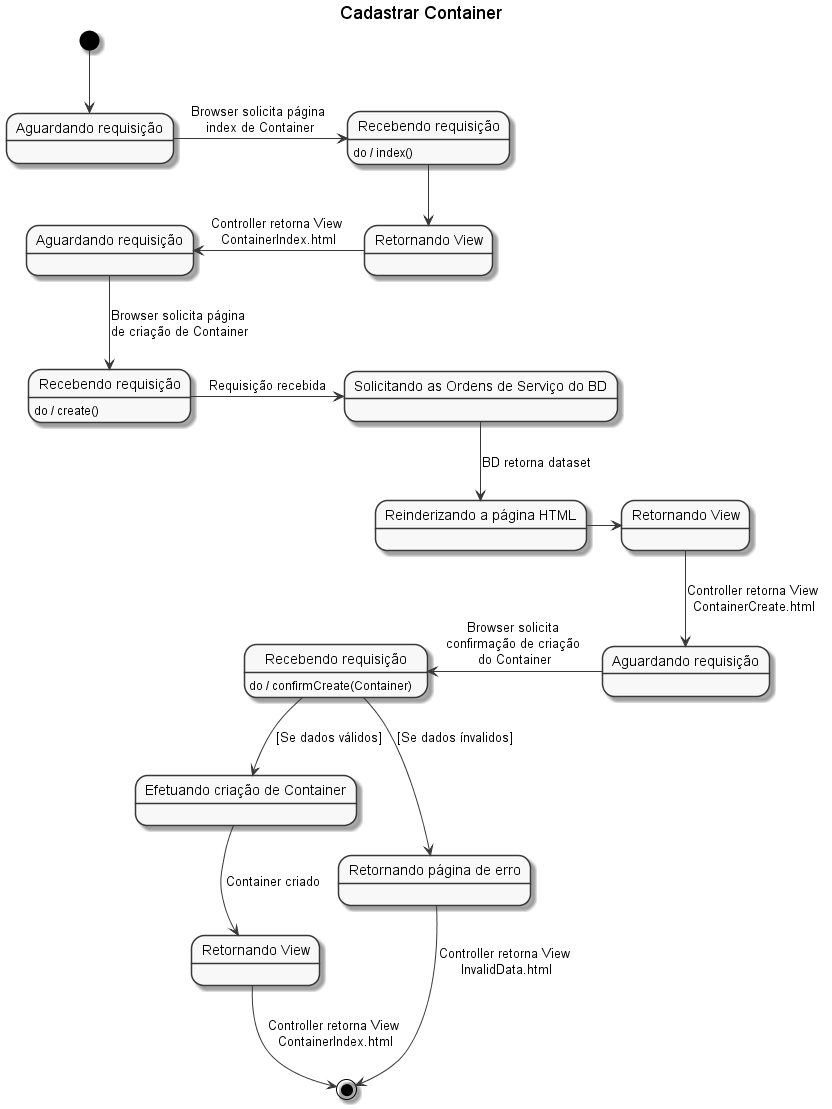
\includegraphics[width=\textwidth]{./Images/DE_-_Cadastrar_Container.png}
    \caption{Diagrama de Estados 12}
    \label{fig:diag_est12}
\end{figure}


\subsection{Inserir Recebimento de Container}

A classe responsável pela troca de estados neste diagrama é a ContainersController, a qual deve retornar ao usuário a lista com todos os containers, seus respectivos materiais e quantidades agrupadas para permitir que o usuário selecione e cadastre um novo ajuste positivo de estoque no sistema. Após recebidas as informações o controlador deve registrar no banco de dados o ajuste e redirecionar o usuário para a página principal da plataforma.

\begin{figure}[H]
    \centering
    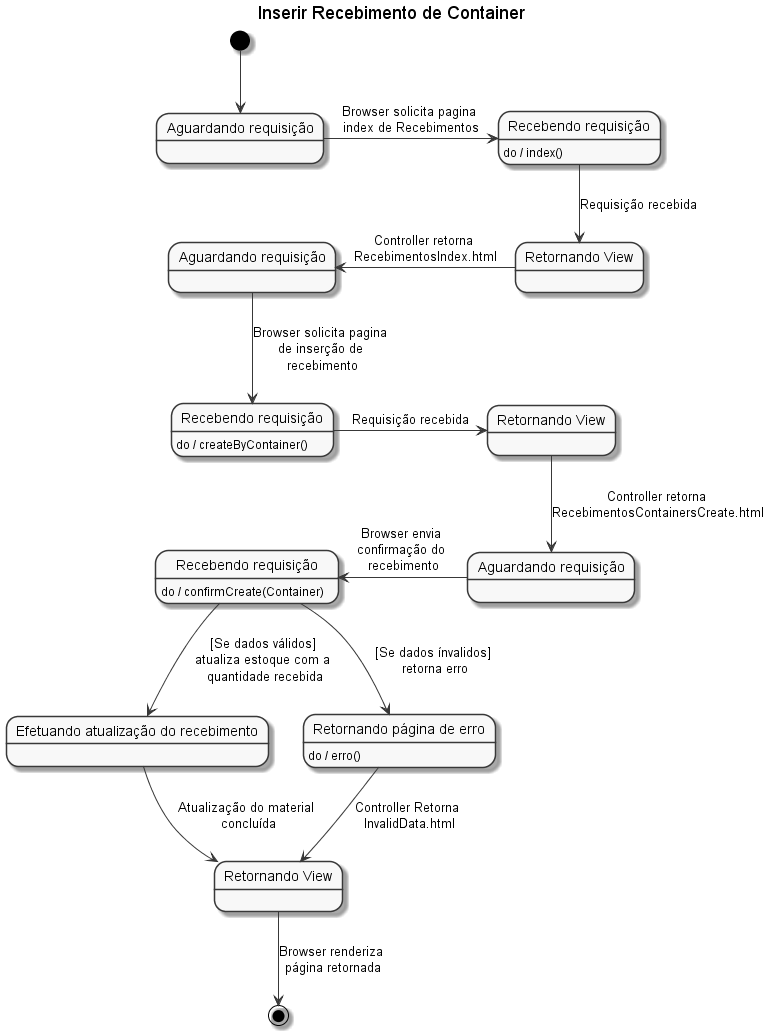
\includegraphics[scale=0.6, width=400pt]{./Images/DE_-_Inserir_Recebimento_de_Container.png}
    \caption{Diagrama de Estados 13}
    \label{fig:diag_est13}
\end{figure}

\subsection{Atualizar Cadastro de Material}

Neste cenário, o controlador representado é o MateriaisController, o qual deve retornar ao usuário a página de edição de cadastro de materiais após selecionado o número do material que se deseja alterar. Então, quando recebido o formulário editado o controlador deve cadastrar no banco de dados as alterações fornecidas e redirecionar o usuário novamente à página principal do sistema.

\begin{figure}[H]
    \centering
    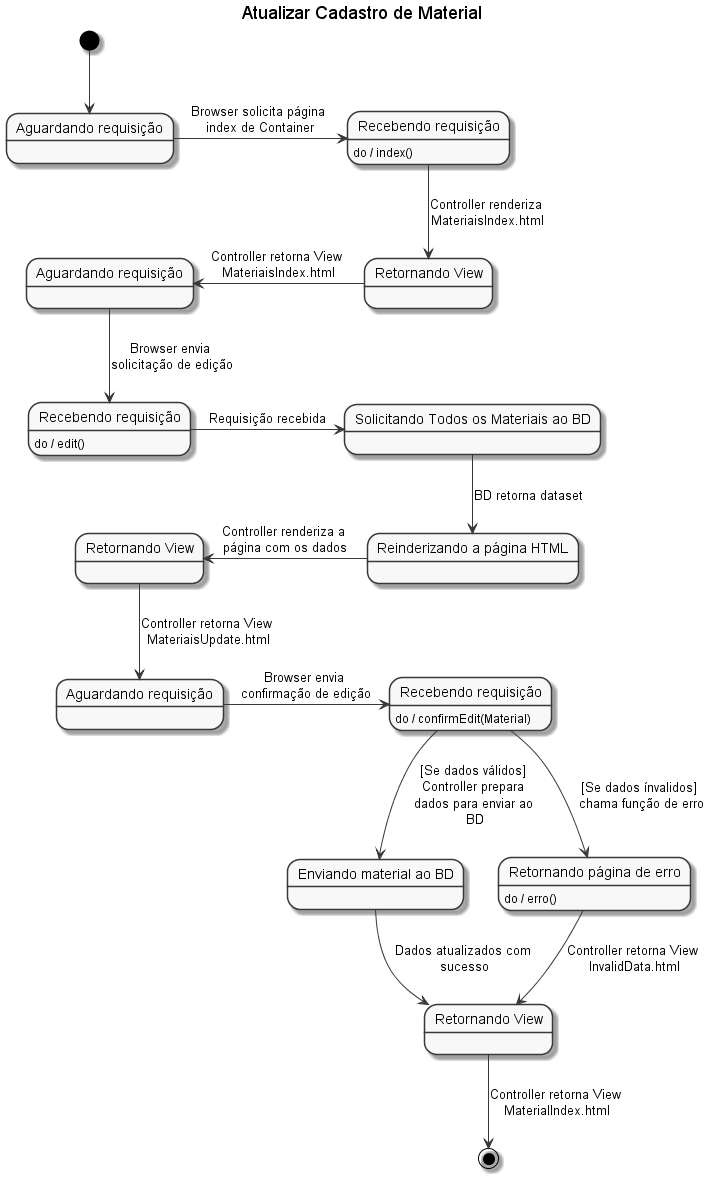
\includegraphics[scale=0.6, width=350pt]{./Images/DE_-_Atualizar_Cadastro_de_Material.png}
    \caption{Diagrama de Estados 14}
    \label{fig:diag_est14}
\end{figure}

\subsection{Atualizar Cadastro de Container}

Esse diagrama retrata o comportamento da classe ContainersController, que espera do usuário uma requisição para processar uma View com o formulário de atualização. Após o preenchimento desse formulário pelo usuário, é feita uma requisição de confirmação para o sistema, e o controller responsável processa a requisição para persistir essa atualização no banco de dados.

\begin{figure}[H]
    \centering
    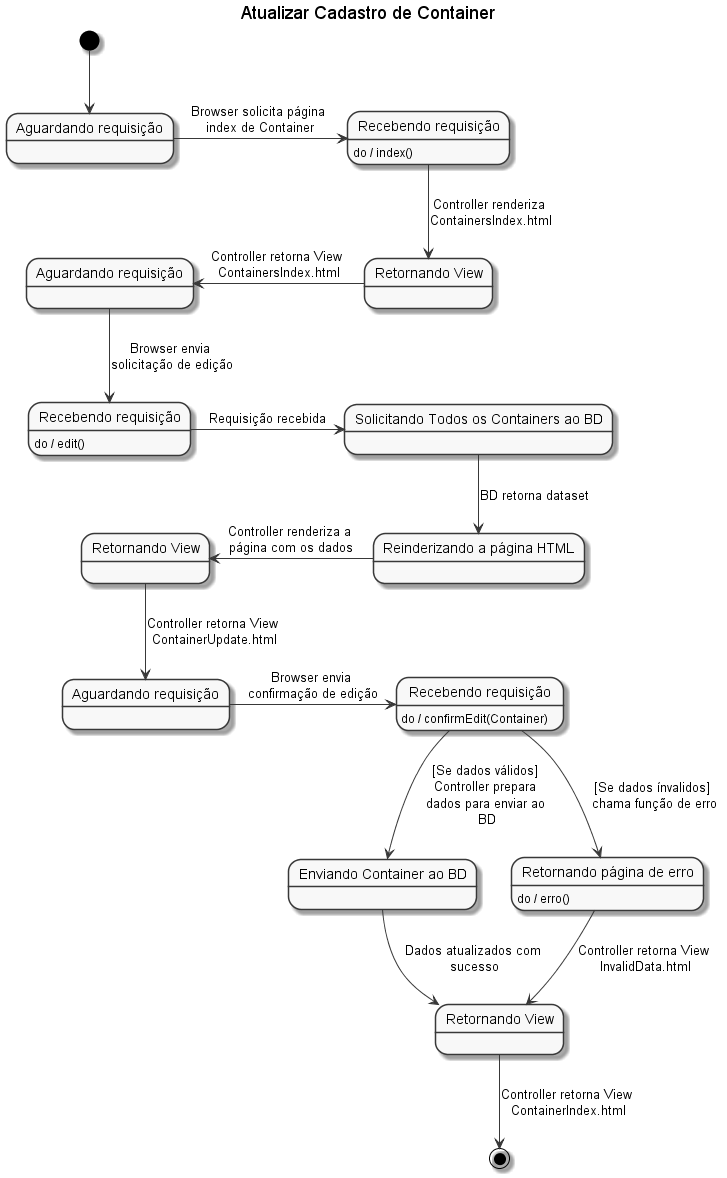
\includegraphics[scale=0.6, width=350pt]{./Images/DE_-_Atualizar_Cadastro_de_Container.png}
    \caption{Diagrama de Estados 15}
    \label{fig:diag_est15}
\end{figure}

\pagebreak

\section{Diagrama de Atividades} \label{diagramaAtividade}

O Diagrama de Atividades é comumente utilizado para representação de fluxos dentro dos softwares, seja para especificações de baixo nível referentes à implementação de funcionalidades, ou para a representação do fluxo de negócio de um sistema, assim exibindo de forma mais geral o workflow da regra de negócio atendida.

Nos diagramas abaixo estão representados os fluxos de negócio para cada um dos casos de uso definidos no sistema. Sendo que o fluxo representado inicialmente representa um workflow que engloba a utilização de todos os demais diagramas de atividades, servindo como um aspecto geral de funcionamento do sistema na companhia.

O diagrama principal, denominado "Processo Produtivo" foi segmentado em 5 partes a fim de melhorar sua visualização. A separação de cada porção do diagrama foi feita utilizando o conceito de Conectores no diagrama de atividades, os quais representam links diretos entre diferentes atividades.

\subsection{Processo Produtivo - Parte 1}

\begin{figure}[H]
    \centering
    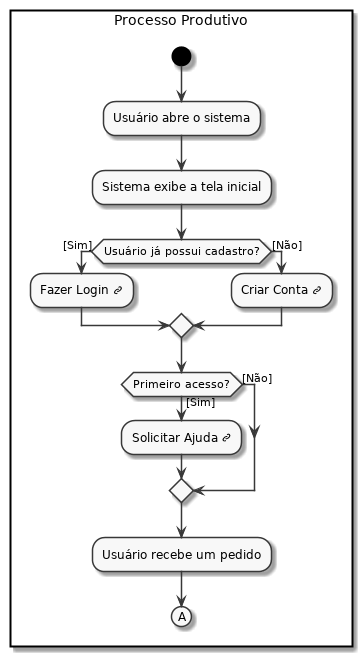
\includegraphics[scale=0.6, width=300pt]{./Images/DA_Processo_Produtivo.png}
    \caption{Diagrama de Atividades 1}
    \label{fig:diag_atv1}
\end{figure}

\subsection{Processo Produtivo - Parte 2}

\begin{figure}[H]
    \centering
    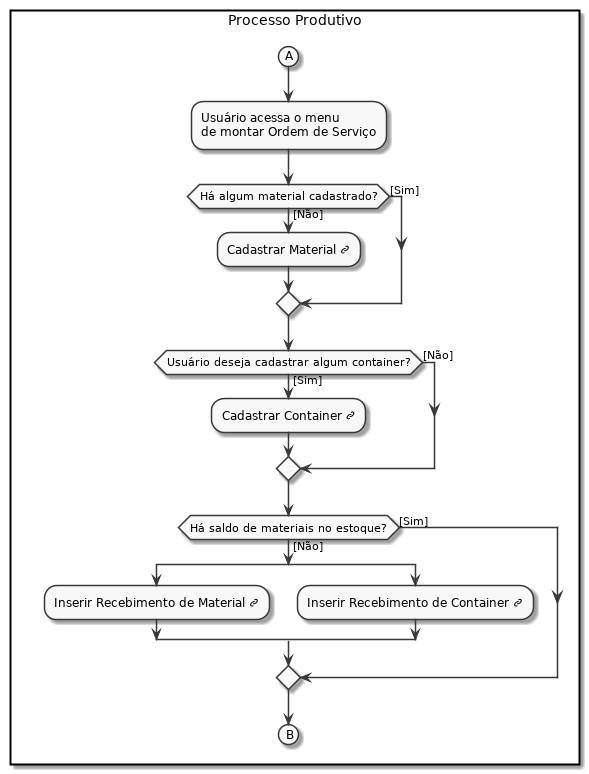
\includegraphics[scale=0.6, width=400pt]{./Images/DA_Processo_Produvito2.png}
    \caption{Diagrama de Atividades 2}
    \label{fig:diag_atv2}
\end{figure}

\subsection{Processo Produtivo - Parte 3}

\begin{figure}[H]
    \centering
    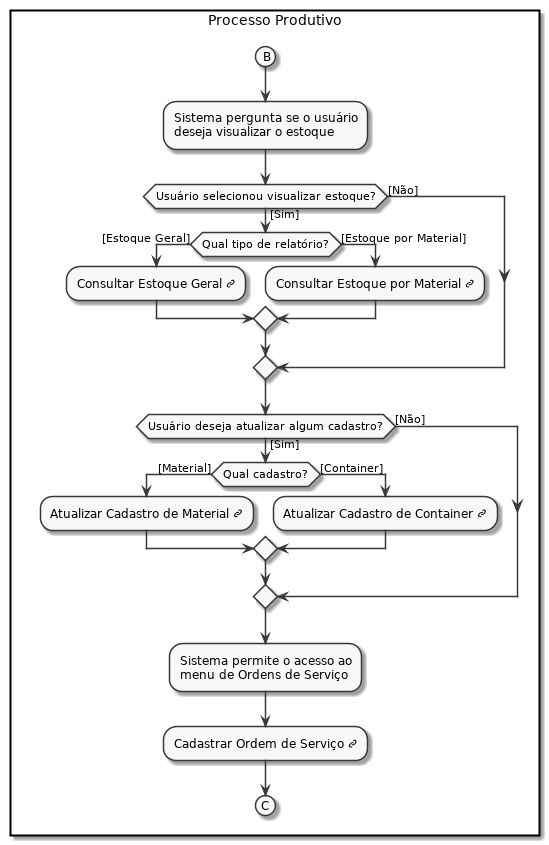
\includegraphics[scale=0.6, width=400pt]{./Images/DA_Processo_Produtivo3.png}
    \caption{Diagrama de Atividades 3}
    \label{fig:diag_atv3}
\end{figure}

\subsection{Processo Produtivo - Parte 4}

\begin{figure}[H]
    \centering
    \includegraphics[scale=0.6, width=400pt]{./Images/DA_Processo_Produtivo4.png}
    \caption{Diagrama de Atividades 4}
    \label{fig:diag_atv4}
\end{figure}

\subsection{Processo Produtivo - Parte 5}

\begin{figure}[H]
    \centering
    \includegraphics[scale=0.6, width=300pt]{./Images/DA_Processo_Produtivo5.png}
    \caption{Diagrama de Atividades 5}
    \label{fig:diag_atv5}
\end{figure}

\subsection{Cadastrar Material}

\begin{figure}[H]
    \centering
    \includegraphics[scale=0.6, width=400pt]{./Images/Cadastrar_Material.png}
    \caption{Diagrama de Atividades 6}
    \label{fig:diag_atv6}
\end{figure}

\subsection{Consultar Estoque Geral}

\begin{figure}[H]
    \centering
    \includegraphics[scale=0.6, width=400pt]{./Images/Consultar_Estoque_Geral.png}
    \caption{Diagrama de Atividades 7}
    \label{fig:diag_atv7}
\end{figure}

\subsection{Inserir Baixa de Material}

\begin{figure}[H]
    \centering
    \includegraphics[scale=0.6, width=400pt]{./Images/Inserir_Baixa_de_Material.png}
    \caption{Diagrama de Atividades 8}
    \label{fig:diag_atv8}
\end{figure}

\subsection{Inserir Recebimento de Material}

\begin{figure}[H]
    \centering
    \includegraphics[scale=0.6, width=400pt]{./Images/Inserir_Recebimento_de_Material.png}
    \caption{Diagrama de Atividades 9}
    \label{fig:diag_atv9}
\end{figure}

\subsection{Fazer Login}

\begin{figure}[H]
    \centering
    \includegraphics[scale=0.6, width=300pt]{./Images/Fazer_Login.png}
    \caption{Diagrama de Atividades 10}
    \label{fig:diag_atv10}
\end{figure}

\subsection{Criar Conta}

\begin{figure}[H]
    \centering
    \includegraphics[scale=0.6, width=300pt]{./Images/Criar_Conta.png}
    \caption{Diagrama de Atividades 11}
    \label{fig:diag_atv11}
\end{figure}

\subsection{Solicitar Ajuda}

\begin{figure}[H]
    \centering
    \includegraphics[scale=0.6, width=300pt]{./Images/Solicitar_Ajuda.png}
    \caption{Diagrama de Atividades 12}
    \label{fig:diag_atv12}
\end{figure}

\subsection{Consultar Estoque por Material}

\begin{figure}[H]
    \centering
    \includegraphics[scale=0.6, width=400pt]{./Images/Consultar_Estoque_por_Material.png}
    \caption{Diagrama de Atividades 13}
    \label{fig:diag_atv13}
\end{figure}

\subsection{Cadastrar Necessidade de Material}

\begin{figure}[H]
    \centering
    \includegraphics[scale=0.6, width=300pt]{./Images/Cadastrar_Necessidade_de_Material.png}
    \caption{Diagrama de Atividades 14}
    \label{fig:diag_atv14}
\end{figure}

\subsection{Cadastrar Ordem de Serviço}

\begin{figure}[H]
    \centering
    \includegraphics[scale=0.6, width=200pt]{./Images/Cadastrar_Ordem_de_Servico.png}
    \caption{Diagrama de Atividades 15}
    \label{fig:diag_atv15}
\end{figure}

\subsection{Finalizar Ordem de Serviço}

\begin{figure}[H]
    \centering
    \includegraphics[scale=0.6, width=200pt]{./Images/Finalizar_Ordem_de_Servico.png}
    \caption{Diagrama de Atividades 16}
    \label{fig:diag_atv16}
\end{figure}


\subsection{Cadastrar Container}

\begin{figure}[H]
    \centering
    \includegraphics[scale=0.6, width=400pt]{./Images/Cadastrar_Container.png}
    \caption{Diagrama de Atividades 17}
    \label{fig:diag_atv17}
\end{figure}

\subsection{Inserir Recebimento de Container}

\begin{figure}[H]
    \centering
    \includegraphics[scale=0.6, width=300pt]{./Images/Inserir_Recebimento_de_Container.png}
    \caption{Diagrama de Atividades 18}
    \label{fig:diag_atv18}
\end{figure}

\subsection{Atualizar Cadastro de Material}

\begin{figure}[H]
    \centering
    \includegraphics[scale=0.6, width=400pt]{./Images/Atualizar_Cadastro_de_Material.png}
    \caption{Diagrama de Atividades 19}
    \label{fig:diag_atv19}
\end{figure}

\subsection{Atualizar Cadastro de Container}

\begin{figure}[H]
    \centering
    \includegraphics[scale=0.6, width=400pt]{./Images/Atualizar_Cadastro_de_Container.png}
    \caption{Diagrama de Atividades 20}
    \label{fig:diag_atv20}
\end{figure}


\section{Diagrama de Componentes} \label{diagramaComp}

O Diagrama de Componentes procura modelar a representação de cada um dos módulos que constituirão o sistema em sua fase de implementação e está diretamente associado à linguagem e paradigma de programação utilizados para seu desenvolvimento.

Os diagramas a seguir representam como o sistema foi segmentado de acordo com a arquitetura MVC (Model - View - Controller), muito utilizada atualmente para facilitar e compartimentalizar cada componente utilizado no desenvolvimento de softwares baseados na Web, bem como a arquitetura definida para o Banco de Dados que realizará a persistência dos dados da aplicação.

\subsection{Diagrama de Caixa Preta}

Este diagrama é utilizado para representar de forma geral a definição e interligação dos principais componentes do sistema, bem como suas interfaces requeridas e fornecidas de comunicação.

No caso abaixo, o servidor de aplicação que executará a regra de negócio do sistema foi representado pelo nome "StockMap.exe", o qual contém como componentes internos as pastas definidas pela arquitetura MVC. Ao seu lado está representada a base de dados denominada "Database", dado que pode-se utilizar qualquer gerenciador de banco de dados relacional (RDBMS), como SQL Server, MySQL, Oracle, entre outros.

\begin{figure}[H]
    \centering
    \includegraphics[scale=0.6, width=400pt]{./Images/Diagrama_de_Componentes.png}
    \caption{Diagrama de Componentes 1}
    \label{fig:diag_componentes}
\end{figure}

\subsection{Controllers}

Neste diagrama estão representados os controladores definidos para o sistema. Estes serão responsáveis por receber, validar e executar as requisições recebidas pela plataforma, respeitando a regra de negócio e os fluxos estipulados nos diagramas anteriores.

\begin{figure}[H]
    \centering
    \includegraphics[scale=0.6, width=400pt]{./Images/Diagrama_de_Componentes_-_Controllers.png}
    \caption{Diagrama de Componentes 2}
    \label{fig:diag_componentes2}
\end{figure}

\subsection{Views}

Neste diagrama é representada a organização das pastas que contém os arquivos HTML, de visualização do sistema. Estes foram segmentados por cada entidade criada e agrupam as páginas manipuladas pelos controladores para receber e enviar os dados para os usuários.

Abaixo está representada a forma geral de organização das pastas, sendo que serão apresentados os arquivos HTML modelados nos diagramas a seguir.

\begin{figure}[H]
    \centering
    \includegraphics[scale=0.6, width=400pt]{./Images/Diagrama_de_Componentes_-_Views.png}
    \caption{Diagrama de Componentes 3}
    \label{fig:diag_componentes3}
\end{figure}

\subsubsection{Home}

Este diagrama de componentes representa os arquivos de visualização utilizados nas primeiras interações do usuário com o sistema, seja para login, criação de conta ou exibição do menu principal, que concede acesso às demais funcionalidades da plataforma.

\begin{figure}[H]
    \centering
    \includegraphics[scale=0.6, width=400pt]{./Images/Diagrama_de_Componentes_-_Home.png}
    \caption{Diagrama de Componentes 4}
    \label{fig:diag_componentes4}
\end{figure}

\subsubsection{Material}

O diagrama de componentes de Materiais abaixo exibe as páginas HTML utilizadas para gerenciar o controle de estoque e de códigos de materiais do sistema.

\begin{figure}[H]
    \centering
    \includegraphics[scale=0.6, width=400pt]{./Images/Diagrama_de_Componentes_-_Material.png}
    \caption{Diagrama de Componentes 5}
    \label{fig:diag_componentes5}
\end{figure}

\subsubsection{Necessidade de Material}

Neste diagrama de componentes são modelados os documentos criados para permitir que os usuários enviem requisições para criação de notificações de necessidade de material, as quais representam um importante papel no controle de estoque servindo como principal meio de planejamento e controle das produções atuais e futuras na plataforma.

\begin{figure}[H]
    \centering
    \includegraphics[scale=0.6, width=400pt]{./Images/Diagrama_de_Componentes_-_NecessidadeMaterial.png}
    \caption{Diagrama de Componentes 6}
    \label{fig:diag_componentes6}
\end{figure}

\subsubsection{Ordem de Serviço}

O diagrama de componente de ordens de serviço contém as páginas responsáveis por captar dados para criação, finalização, listagem e pesquisa das ordens existentes na plataforma, assim facilitando o controle produtivo e gerenciamento dos materiais utilizados.

\begin{figure}[H]
    \centering
    \includegraphics[scale=0.6, width=400pt]{./Images/Diagrama_de_Componentes_-_OrdemServico.png}
    \caption{Diagrama de Componentes 7}
    \label{fig:diag_componentes7}
\end{figure}

\subsubsection{Recebimento}

Os componentes de recebimento são necessários para registrar a inserção de material em estoque tanto de forma individual, quando pelos containers, que representam um conjunto pré-definido de materiais, para facilitar o cadastro em estoque.

\begin{figure}[H]
    \centering
    \includegraphics[scale=0.6, width=400pt]{./Images/Diagrama_de_Componentes_-_Recebimento.png}
    \caption{Diagrama de Componentes 8}
    \label{fig:diag_componentes8}
\end{figure}

\subsection{Models}

Neste diagrama são representados os arquivos de código-fonte que servirão de base para criação das entidades utilizadas pelo sistema e persistidas pelo banco de dados.

\begin{figure}[H]
    \centering
    \includegraphics[scale=0.6, width=400pt]{./Images/Diagrama_de_Componentes_-_Models.png}
    \caption{Diagrama de Componentes 9}
    \label{fig:diag_componentes3}
\end{figure}

\section{Diagrama de Implatação} \label{diagramaImp}

O Diagrama de Implantação é utilizado para projetar a construção física necessária para a execução do software desenvolvido, podendo determinar requisitos de computadores, servidores, protocolos, entre outros.

No diagrama abaixo os componentes definidos para o sistema foram segmentados em dois servidores, um dedicado para executar o gerenciados de banco de dados, o qual deve fornecer uma interface de comunicação - geralmente um driver ODBC - para troca de dados com o segundo servidor, denominado servidor de aplicação, responsável por executar a aplicação com as definições dadas anteriormente.

\begin{figure}[H]
    \centering
    \includegraphics[width=\textwidth]{./Images/Diagrama_de_Implant.png}
    \caption{Diagrama de Implantação}
    \label{fig:diag_implant}
\end{figure}

\printbibliography

%\printindex

\end{document}

